\documentclass[pdflatex,sn-nature]{sn-jnl}% Style for submissions to Nature Portfolio journals

\usepackage{graphicx}%
\usepackage{multirow}%
\usepackage{amsmath,amssymb,amsfonts}%
\usepackage{amsthm}%
\usepackage{mathrsfs}%
\usepackage[title]{appendix}%
\usepackage{xcolor}%
\usepackage{textcomp}%
\usepackage{manyfoot}%
\usepackage{booktabs}%
\usepackage{threeparttable}
\usepackage{siunitx}
\usepackage{caption}
\usepackage{algorithm}%
\usepackage{algorithmicx}%
\usepackage{algpseudocode}%
\usepackage{listings}%
\usepackage{hyperref}%
\usepackage{placeins}%
\usepackage{marginnote}%
\setlength{\marginparwidth}{1.8cm}%
\renewcommand*{\marginfont}{\tiny\sffamily\bfseries\color{blue}}%
\newcommand{\revtag}[1]{\marginnote{#1}}%

%%%%
\theoremstyle{thmstyleone}%
\newtheorem{theorem}{Theorem}%  meant for continuous numbers
%%\newtheorem{theorem}{Theorem}[section]% meant for sectionwise numbers
%% optional argument [theorem] produces theorem numbering sequence instead of independent numbers for Proposition
\newtheorem{proposition}[theorem]{Proposition}% 
%%\newtheorem{proposition}{Proposition}% to get separate numbers for theorem and proposition etc.
\newcommand{\norm}[1]{\left\|#1\right\|}
\theoremstyle{thmstyletwo}%
\newtheorem{example}{Example}%
\newtheorem{remark}{Remark}%

\theoremstyle{thmstylethree}%
\newtheorem{definition}{Definition}%

\raggedbottom
%%\unnumbered% uncomment this for unnumbered level heads

\begin{document}

\title[Integrating Fundamental Knowledge and Sensor Data: Physics-Informed Neural Networks for Smart Agricultural Water Management]{Integrating Fundamental Knowledge and Sensor Data: Physics-Informed Neural Networks for Smart Agricultural Water Management}






\author*[1]{\fnm{Gregory} \sur{Conde}}\email{gregory.condemen@ufl.edu}

\author[1]{\fnm{Sandra M.} \sur{Guzmán}}\email{sandra.guzmangut@ufl.edu}

\author[2]{\fnm{Jorge I.} \sur{Poveda}}\email{jipoveda@ucsd.edu}

\author[3]{\fnm{Flavia T.} \sur{Zambon}}\email{f.zambon@ufl.edu}


\affil*[1]{\orgdiv{Agricultural and Biological Engineering, Indian River Research and Education Center}, \orgname{University of Florida}, \orgaddress{\city{Fort Pierce}, \postcode{34945}, \state{Florida}, \country{USA}}}

\affil[2]{\orgdiv{Department of Electrical and Computer Engineering}, \orgname{University of California}, \orgaddress{\city{San Diego}, \postcode{92093}, \state{California}, \country{USA}}}

\affil[3]{\orgdiv{Institute of Food and Agricultural Sciences, Indian River Research and Education Center}, \orgname{University of Florida}, \orgaddress{\city{Fort Pierce}, \postcode{34945}, \state{Florida}, \country{USA}}}



%%==================================%%
%% Sample for unstructured abstract %%
%%==================================%%
\abstract{Agriculture accounts for 70\% of global freshwater use, yet irrigation inefficiency threatens food security as water scarcity intensifies. Accurate soil moisture prediction for decision-making is crucial for sustainable water management in horticultural systems; however, traditional approaches face an unresolved challenge: analytical models {\color{blue}\marginnote{E-1.1, R-1.3d}require site-specific constitutive calibration, while unconstrained data-driven methods can exhibit physically reversed or non-monotonic responses to irrigation and evaporative demand, undermining reliable predictive} control decisions. Here, we present a physics-informed neural network (PINN) that addresses this by embedding the principles of Richards' equation into a deep learning architecture, enabling control-oriented modeling and decision-making in irrigation systems. The PINN discretizes Richards' equation spatially, modeling flow through {\color{blue}physically regularized} neural branches that yield ordinary differential equations at sensor depths. Trained {\color{blue}\marginnote{R-2.1, R-2.8}in two stages---derivative-matching initialization followed by multi-step fourth-order Runge--Kutta (RK4) trajectory refinement---}the model predicts soil moisture {\color{blue}\marginnote{E-1.1, R-1.3a, R-2.6, R-2.10, R-2.11}across six depths (5--55~\si{cm}) in a commercial Florida citrus block with an overall 3-day held-out forecast RMSE of \SI{1.23}{\%VWC} ($R^2 = 0.807$, Pearson $r = 0.921$, $p = \num{7.94e-178}$; $\approx\SI{3.22}{mm}$ of equivalent water variation integrated over the 60-\si{cm} profile) while simultaneously inferring depth-resolved evapotranspirative depletion. Ablation and baseline comparisons confirm that the proposed PINN reduces 3-day forecast error by 35.6\% over persistence, outperforms single-stage and unregularized variants, and avoids the physically reversed irrigation and evapotranspiration responses exhibited by unconstrained baselines, providing an interpretable model suitable for future model-predictive irrigation control.}}

%\keywords{Water, Smart Irrigation, Physics Informed Neural Networks, PINN, Modeling, Soil Moisture, Richards' equation}





\maketitle

Agriculture consumes 70\% of global freshwater\cite{scanlon2023}, yet irrigation efficiency remains below 50\% in many regions\cite{Mehta2024}, resulting in the wasteful use of a resource essential for food security. Smart irrigation systems, which utilize sensors and algorithms to optimize water delivery, offer a solution; however, \marginnote{E-1.1, R-1.1, R-1.2, R-1.3d}\textcolor{blue}{while recent machine-learning, time-series, and lumped water-balance frameworks already integrate historical soil water content (SWC), weather variables, and uncertainty estimates for soil moisture forecasting and irrigation scheduling~\cite{Zou2010, Murcia2024, Bagheri2025, condeforecast2024}, existing approaches force a trade-off between black-box predictors that can violate physical conservation and actuation laws, lumped control models that lose vertical root-zone resolution, and mechanistic Richards' solvers~\cite{Celia1990, swap2024} that require site-specific hydraulic calibration---leaving multi-depth models that are simultaneously physically consistent and structurally tractable for model predictive control (MPC) an open challenge.} The result is irrigation management that remains largely reactive rather than anticipatory, missing opportunities to reduce water use while maintaining crop productivity.

%--- Move 2: Practical & Scientific Gaps --------------------------------------

The technical gap is well-defined. Smart irrigation algorithms are necessary to pinpoint the precise locations where water should be supplied as plant root systems develop. During germination, water must reach the topsoil layers where seeds are planted; as crops develop, deeper soil layers become critical. Although studies provide general depth guidelines for certain crop types \cite{ASABE2021}, the ability to precisely locate where plants require water based on real-time crop data remains elusive. Algorithms must account for how irrigation, rainfall, plant water uptake, and environmental conditions collectively influence soil water content (SWC) across depths, ideally integrating weather forecasts to predict soil moisture response to upcoming irrigation events. Current approaches fall short: one method uses potential evapotranspiration and crop coefficients to calculate water requirements \cite{Volk2024}; another irrigates based on sensor thresholds between field capacity and maximum allowable depletion \cite{zhang2021}.\marginnote{E-1.1, R-1.1} Neither incorporates current soil moisture, anticipated dynamics, predicted rainfall, and projected crop demands \textcolor{blue}{across multiple soil depths, and even recent predictive scheduling models treat the root zone as a single layer or single sensor point~\cite{Bagheri2025, condeforecast2024} rather than modeling how applied irrigation and crop uptake evolve by depth.}
The modeling challenge is formidable. Capturing plant-soil-water interactions at multiple depths requires confronting: (i) the dynamic nature of plant growth and water uptake, which varies with crop type, phenology, and environmental conditions; (ii) the nonlinearity of Richards' equation governing vertical water movement in unsaturated soils, which demands complex numerical methods \cite{Celia1990}; (iii) the empirical constitutive models (e.g., Gardner, van Genuchten, Brooks–Corey) that represent gravitational and capillary forces in Richards' equation, requiring labor-intensive parameter calibration and lacking universal applicability across soil types \cite{Pan2019}; and (iv) the coarse spatial and temporal resolution of available data, which forces discretizations that can violate numerical stability criteria \cite{Celia1990,leveque2007}. Traditional analytical models are computationally expensive and require soil hydraulic parameters that vary unpredictably in heterogeneous fields. Purely data-driven machine learning models can predict soil moisture \marginnote{R-1.3d}\textcolor{blue}{accurately in-distribution}, but they produce "black box" outputs that \textcolor{blue}{can exhibit physically reversed or non-monotonic responses to irrigation and evapotranspiration inputs and} lack the physical consistency and stability guarantees necessary for model predictive control.

%--- Move 3: Opportunity & Approach -------------------------------------------
Here, we address this dichotomy with physics-informed neural networks (PINNs), a technique that combines neural network function approximation, machine learning tools, established soil-water dynamics theory, and plant biophysics into models suitable for smart irrigation management. Originally created to reduce computational costs when solving partial differential equations (PDEs)  \cite{Cuomo2022}, PINNs \marginnote{E-1.1}\textcolor{blue}{offer a pathway to} overcome the limitations of purely data-driven approaches (which require vast data and lack physical consistency) and analytical models (which are computationally expensive and depend on system-specific governing equations).


%--- Move 4: Prior Art & Positioning
Recent applications demonstrate the potential of PINNs for control-oriented modeling in high-uncertainty systems, such as automated vehicles and quantum systems \cite{Li2024, Zhang2025}. In soil sciences, PINNs have been explored as alternatives to numerical solutions of Richards' equation \cite{Bandai2022}, for handling sparse data in unsaturated infiltration modeling \cite{Lan2024}, for estimating hydraulic conductivity functions \cite{Elkha2024}, and for predicting SWC \cite{Bagheri2025}. \marginnote{E-1.1, R-1.1, R-2.1}\textcolor{blue}{However, enabling predictive irrigation control across a root zone requires five capabilities simultaneously (Table~\ref{tab:lit_comparison}): multi-depth sensor resolution, learning without prescribed soil-retention curves, explicit irrigation and weather inputs, depth-resolved depletion interpretability, and physically consistent multi-step responses. Existing studies satisfy only subsets of these requisites across three spaces: physics-informed Richards' surrogates~\cite{Bandai2022, Lan2024, Elkha2024, Bandai2024, Ye2025} omit crop sinks and irrigation control inputs; data-driven and physics-guided forecasters~\cite{Zou2010, Murcia2024, Bagheri2025, WangY2023, ZhangT2025, Jiang2025, Jiang2026} lack decomposed fluxes and physical response guarantees under sparse field data; and control-oriented water-balance models~\cite{condeforecast2024} lump the root zone into a single layer.}

%--- Move 5: Research Questions and work 
\textcolor{blue}{To\marginnote{R-2.1} bridge this gap, we} ask: Can PINNs that incorporate principles of Richards' equation and sensor data effectively model plant-soil-water dynamics to \marginnote{E-1.1, R-2.6, R-2.8, R-2.11}\textcolor{blue}{support predictive irrigation control} and spatially localize crop water demands? Can such models be physically interpretable and useful for decision-making? \textcolor{blue}{First, we} use Richards' equation as a structural framework, spatially discretizing it at sensor depths throughout the soil profile \textcolor{blue}{without prescribed soil-retention curves} to obtain differential equations that describe the dynamics and relationships of each soil layer with irrigation \textcolor{blue}{($q_{\mathrm{irr}}$)}, rainfall \textcolor{blue}{($r$)}, and potential evapotranspiration ($ET_0$), as flow functions that satisfy water balance constraints. \textcolor{blue}{Evapotranspirative water depletion} appears as a sink function of $ET_0$ and soil moisture at each layer. \textcolor{blue}{Second, all} flow functions are approximated using \textcolor{blue}{decomposed} neural network branches that are \textcolor{blue}{regularized} for physical consistency (non-negativity, monotonicity, and zero\textcolor{blue}{-forcing zero-flux}). \textcolor{blue}{Third, the} PINN is trained in two stages: initially, it minimizes errors against measured soil moisture variations, followed by tuning through the incorporation of the \textcolor{blue}{fourth-order Runge--Kutta (RK4)} numerical solution into the cost function. We validate this approach using field data from citrus production in Florida, where shallow sandy soils and saltwater intrusion create challenging conditions\marginnote{E-1.1, R-1.2, R-1.3d, R-2.10}\textcolor{blue}{, achieving a 3-day forecast root-mean-square error (RMSE) of \SI{1.23}{\%} volumetric water content (\si{\%VWC}) while outperforming ablated variants and preserving physically consistent control responses unavailable in unconstrained baselines.}

\begin{table}[!htbp]
\centering
\marginnote{R-1.1, R-2.1}\caption{\textcolor{blue}{Comparison of modeling families against the five core requisites for multi-depth predictive irrigation management.}}
\label{tab:lit_comparison}
\scriptsize
\setlength{\tabcolsep}{2.2pt}
{\color{blue}\begin{tabular*}{\textwidth}{@{\extracolsep{\fill}}>{\raggedright\arraybackslash}p{0.25\textwidth}>{\raggedright\arraybackslash}p{0.12\textwidth}ccccc@{}}
\toprule
\textbf{Modeling Family} & \textbf{Studies} & \textbf{Multi-} & \textbf{No Soil-} & \textbf{Explicit} & \textbf{Depth} & \textbf{Physically} \\
 & & \textbf{Depth} & \textbf{Curve} & \textbf{Irrig.} & \textbf{Fluxes \&} & \textbf{Consistent} \\
 & & \textbf{Profile} & \textbf{Calib.} & \textbf{Input} & \textbf{Depletion} & \textbf{Control} \\
\midrule
Analytical Richards' PDE models & \cite{Celia1990, swap2024} & $\checkmark$ & $\times$ & $\checkmark$ & $\checkmark$ & Partial$^{\mathrm{a}}$ \\
Physics-informed PDE \& operator surrogates & \cite{Bandai2022, Lan2024, Elkha2024, Bandai2024, Ye2025} & $\checkmark$ & Partial & $\times$ & $\times$ & $\times$ \\
Data-driven time-series \& ML forecasters & \cite{Zou2010, Murcia2024, Bagheri2025} & Partial & $\checkmark$ & $\times$ & $\times$ & $\times$ \\
Physics-guided sequence \& assimilation models & \cite{WangY2023, ZhangT2025, Jiang2025, Jiang2026} & $\checkmark$ & $\times$ & $\times$ & $\times$ & $\times$ \\
Control-oriented lumped water balance & \cite{condeforecast2024} & $\times$ & $\checkmark$ & $\checkmark$ & Partial$^{\mathrm{b}}$ & $\checkmark$ \\
\midrule
\textbf{Proposed sensor-depth PINN} & \textbf{This study} & \boldmath$\checkmark$ & \boldmath$\checkmark$ & \boldmath$\checkmark$ & \boldmath$\checkmark$ & \boldmath$\checkmark$ \\
\bottomrule
\end{tabular*}}
\begin{tablenotes}
\footnotesize
\item \textcolor{blue}{$^{\mathrm{a}}$Physically consistent, but iterative nonlinear PDE solving is computationally demanding for online MPC.}
\item \textcolor{blue}{$^{\mathrm{b}}$Separates lumped rainfall, evapotranspiration, and drainage gains, but without vertical depth localization.}
\end{tablenotes}
\end{table}

%%%%%%%%%%%%%%%%

\section{Results}\label{Results}
%/mnt/ssd/PINNSMb/mainresults.ipynb

\textcolor{blue}{We\marginnote{R-1.4, R-2.9} evaluate the proposed PINN using hourly field telemetry ($\Delta t = \SI{1}{h}$, matching operational weather-forecast resolution~\cite{NWS2024}) from a commercial Florida citrus block planted on raised sandy beds over a shallow clay horizon ($\approx\SI{30}{cm}$) flanked by drainage ditches (Section~\ref{Test Case}, Fig.~\ref{fig:bed_ditch}). As detailed in Section~\ref{Methodology}, six capacitive sensors monitor 10-\si{cm} vertical compartments centered at 5, 15, 25, 35, 45, and 55~\si{cm}, where layer water balances are modeled by physically regularized neural flux branches trained in two stages.}

\begin{figure}[!htbp]
\centering
\includegraphics[width=\linewidth]{estimation_vs_validation_with_plant_uptake.pdf}
\marginnote{R-1.2, R-2.3, R-2.4, R-2.6, R-2.12}\caption{\textcolor{blue}{Evaluation of the proposed PINN for multi-depth soil moisture prediction, showing measured rainfall ($r$, \si{mm/h}), irrigation duration fraction ($q_{\mathrm{irr}}$, \si{h/h}), FAO-56 Penman--Monteith evapotranspiration ($ET_0$, \si{mm/h}), and measured versus estimated soil moisture (\si{\%VWC}) across 5--55~\si{cm} over the 35-day training period (839~h) and held-out 3-day forecast (72~h, after a 25-h buffer), driven solely by $m(0)$ and observed ($r, q_{\mathrm{irr}}, ET_0$). Moisture heatmaps use a 3.5--10.2~\si{\%VWC} contrast range ($\approx 90\%$ empirical interval; 5.8th--92.1st training percentiles). Lower panels show inferred evapotranspirative depletion rates ($pc_i$, \si{\%VWC/h}).}}
\label{Mainfig}
\end{figure}


The results of the evaluation of the proposed PINN approach are shown in Fig.~\ref{Mainfig}, where rain \textcolor{blue}{($r$)}, irrigation \textcolor{blue}{($q_{\mathrm{irr}}$), reference evapotranspiration ($ET_0$)}, and soil moisture data used during the \textcolor{blue}{35-day} training and \textcolor{blue}{held-out 3-day} forecasting periods are presented. \marginnote{R-1.2, R-2.4, R-2.12}\textcolor{blue}{Throughout this work, soil moisture (SM, used interchangeably with SWC) is quantified as volumetric water content (\si{\%VWC}, liquid water volume per bulk soil volume, $\mathrm{cm^3\,cm^{-3}} \times 100$), while $ET_0$ (\si{mm/h}) quantifies potential atmospheric evaporative demand via the FAO-56 Penman--Monteith equation~\cite{allen1998crop}. In the moisture heatmaps, the 3.5--10.2~\si{\%VWC} color scale spans the dominant $\approx 90\%$ empirical range (5.8th--92.1st training percentiles, enclosing 86.3\% of observations) so transient topsoil storm spikes do not saturate contrast across intermediate depths.} This visualization helps reveal soil-water dynamics not apparent in common one-dimensional plots. The sampling time used for data management, visualization, and modeling was one hour to align with the availability of data from forecasting services \cite{NWS2024}. The heatmap shows soil moisture over time at depths of 5, 15, 25, 35, 45, and 55 \si{cm}; this spatial discretization is dictated by the number of soil moisture sensors available for data collection. The figure also presents the estimated \marginnote{R-2.6}\textcolor{blue}{evapotranspirative depletion rates ($pc_i$)} at the different depths.

Measured data is used to tune the PINN during training, and unseen data is used to validate the model's effectiveness during forecasting. In Fig.~\ref{Mainfig}, \marginnote{R-2.3, R-2.4}\textcolor{blue}{every predicted trajectory across the 35-day training period (839~h) and held-out 3-day forecast (72~h from May~3, 21:00:00, after a 25-h separation buffer) is generated via free-run simulation} using only initial conditions and \textcolor{blue}{observed station} external inputs such as rain, irrigation, and $ET_0$ \textcolor{blue}{(without state assimilation)}, validating our proposed PINN as a control-oriented model, where the states depend on available measurable and actionable inputs. The figure illustrates the direct impact of external events on both measured and estimated soil moisture levels during the training and forecasting phases. In the upper layers, increases in soil moisture are directly associated with rainfall and irrigation events, while decreases are correlated with rises in measured $ET_0$.

Fig.~\ref{Mainfig} clearly shows that the estimated soil moisture is correlated with the measured soil moisture during both periods. We highlight that: (i) the proposed PINN demonstrates stability, with estimated soil moisture remaining around the measured values during both periods, avoiding divergence toward unphysical values; (ii) the estimated soil moisture across various layers exhibits increases and decreases that are correlated with measured values; (iii) the PINN effectively captures most of the rapid, high soil moisture increases in the first and second layers, though it tends to be conservative in representing such peaks in the deeper layers; and (iv) an anomaly around April 8, where, unlike other rainfall events, this event only caused an increase in the first soil layer. This reflects the variability inherent in these natural systems over relatively short periods, with most of the rainfall appearing to become runoff in this particular event. This may partly explain why the PINN’s estimations are conservative regarding soil moisture peaks at the deepest layers. Another factor contributing to this conservative performance is the selected sampling period. For the first and second layers, peak responses occur approximately two hours following a rainfall or irrigation event. According to classical analyses of discrete systems, it is recommended to select a sampling interval roughly ten times shorter than the system's response time \cite{Franklin1998}. Despite limited data availability, the proposed approach provides an accurate representation of the studied system, underscoring the PINN's robustness in adapting to limited real-world data and environmental conditions.

The model simultaneously estimates \marginnote{R-2.6}\textcolor{blue}{evapotranspirative water depletion ($pc_i$)} at each depth as a function of soil moisture and $ET_0$. This estimation enables the development of more precise control strategies by helping localize depths where soil moisture must be guaranteed. In Fig.~\ref{Mainfig}, the estimated \textcolor{blue}{depletion rates} from 5 to 55 \si{cm} depths \textcolor{blue}{are} illustrated. The results show \textcolor{blue}{depletion} patterns correlated with both soil moisture and $ET_0$ across all layers. The estimation is performed in units of \si{\%VWC/h}, indicating how much soil moisture decreases over time in relation to soil moisture and $ET_0$. \textcolor{blue}{Pronounced maxima} are estimated at the first layer (5 \si{cm}) and the lowest layer (55 \si{cm}), \textcolor{blue}{reflecting non-transpirative surface evaporation at 5~\si{cm} and ditch/water-table drawdown at 55~\si{cm}, whereas within the upper root zone above the clay horizon, peak apparent depletion occurs} at 25 \si{cm} \textcolor{blue}{(see hydrological and agronomic analysis in Section~\ref{sec:uptake_rationale}).}



%/mnt/ssd/PINNSMb/mainresults.ipynb
\begin{figure}[!htbp]
\centering
\includegraphics[width=\linewidth]{error_analysis_heatmap_boxplot.pdf}
\marginnote{R-1.8}\caption{\textcolor{blue}{Soil moisture prediction residuals ($m_i - \hat{m}_i$, \si{\%VWC}) across 5--55~\si{cm} during the 35-day training and 3-day held-out forecasting periods. Black frames delineate heatmap boundaries against zero-error white regions ($-2.5$ to $11.1$~\si{\%VWC}; red under-prediction, blue over-prediction). Bottom boxplots show near-zero medians and interquartile ranges below 2.5~\si{\%VWC} across all depths.}}
\label{errorfig}
\end{figure}

In \textcolor{blue}{Fig.~\ref{errorfig}}, the estimation error is distributed around zero during training and forecasting\marginnote{R-1.8}\textcolor{blue}{, where the box plots show medians near zero and interquartile ranges below \SI{2.5}{\%VWC} across all depths, with occasional outliers due to the conservative peak response of the PINN}. Error peaks are evident at 5 \si{cm} and 55 \si{cm}; the peaks at 5 \si{cm} are correlated with rain and irrigation events, while the peaks at 55 \si{cm} are correlated with high rain events. The direct influence of rain at deeper layers is related to the terrain configuration, which consists of beds with lateral ditches that collect and drain excess water.

\begin{table}[!htbp]
\centering
\marginnote{E-1.1, R-1.3a, R-1.3b, R-2.5, R-2.12}\caption{Statistical analysis of soil moisture estimation across six soil layers, covering training \textcolor{blue}{(35 days, $839\,\mathrm{h}$/layer)} and forecasting \textcolor{blue}{(3 days, $72\,\mathrm{h}$/layer)} periods. \textcolor{blue}{$\sigma_m$ is the measured standard deviation (\si{\%VWC}),} RMSE is the root-mean-square error in \si{\%VWC}, SD is the \textcolor{blue}{error} standard deviation, $R^2$ is the coefficient of determination\textcolor{blue}{, and $r$ is the Pearson correlation coefficient}. The obtained $p$-values indicate statistical significance ($p < 0.0001$ \textcolor{blue}{via two-sided Student's $t$-test, except $^*p = 0.0038$ at 25~\si{cm} in forecasting}). The overall result is obtained by analyzing the concatenated data from the six soil layers.}
\label{tab:stats_combined}
\footnotesize
\setlength{\tabcolsep}{4.5pt}
\begin{tabular}{@{}lcccccccccc@{}}
\toprule
& \multicolumn{5}{c}{Training} & \multicolumn{5}{c}{Forecasting} \\
\cmidrule(lr){2-6}\cmidrule(l){7-11}
\textcolor{blue}{Depth} & \textcolor{blue}{$\sigma_m$} & RMSE & SD & $R^2$ & \textcolor{blue}{$r$} & \textcolor{blue}{$\sigma_m$} & RMSE & SD & $R^2$ & \textcolor{blue}{$r$} \\
\midrule
5 \si{cm}  & \textcolor{blue}{3.53} & \textcolor{blue}{1.90} & 1.81 & \textcolor{blue}{0.710} & \textcolor{blue}{0.858} & \textcolor{blue}{3.99} & \textcolor{blue}{2.02} & \textcolor{blue}{1.81} & \textcolor{blue}{0.740} & \textcolor{blue}{0.948} \\
15 \si{cm} & \textcolor{blue}{2.16} & \textcolor{blue}{0.91} & 0.90 & \textcolor{blue}{0.821} & \textcolor{blue}{0.910} & \textcolor{blue}{1.47} & \textcolor{blue}{1.11} & 0.99 & \textcolor{blue}{0.417} & \textcolor{blue}{0.802} \\
25 \si{cm} & \textcolor{blue}{1.08} & \textcolor{blue}{0.77} & 0.73 & \textcolor{blue}{0.492} & \textcolor{blue}{0.772} & \textcolor{blue}{0.87} & \textcolor{blue}{1.05} & \textcolor{blue}{0.85} & \textcolor{blue}{$-0.455$} & \textcolor{blue}{$0.337^*$} \\
35 \si{cm} & \textcolor{blue}{0.88} & \textcolor{blue}{0.45} & 0.44 & \textcolor{blue}{0.741} & \textcolor{blue}{0.888} & \textcolor{blue}{0.42} & \textcolor{blue}{0.28} & 0.24 & \textcolor{blue}{0.567} & \textcolor{blue}{0.841} \\
45 \si{cm} & \textcolor{blue}{2.14} & \textcolor{blue}{0.79} & 0.76 & \textcolor{blue}{0.865} & \textcolor{blue}{0.953} & \textcolor{blue}{0.34} & \textcolor{blue}{0.95} & \textcolor{blue}{0.49} & \textcolor{blue}{$-7.043$} & \textcolor{blue}{0.709} \\
55 \si{cm} & \textcolor{blue}{3.09} & \textcolor{blue}{1.47} & 1.40 & \textcolor{blue}{0.772} & \textcolor{blue}{0.934} & \textcolor{blue}{0.17} & \textcolor{blue}{1.32} & 0.64 & \textcolor{blue}{$-59.517$} & \textcolor{blue}{0.713} \\
\midrule
Overall & \textcolor{blue}{2.56} & \textcolor{blue}{1.16} & 1.12 & \textcolor{blue}{0.796} & \textcolor{blue}{0.901} & \textcolor{blue}{2.81} & \textcolor{blue}{1.23} & \textcolor{blue}{1.24} & \textcolor{blue}{0.807} & \textcolor{blue}{0.921} \\
\bottomrule
\end{tabular}
\end{table}

The estimation performance is verified through statistical analyses, presented in Table~\ref{tab:stats_combined}\marginnote{E-1.1, R-1.3a, R-1.3c}\textcolor{blue}{, Fig.~\ref{errorfig}, and the predicted-versus-measured scatterplots in Fig.~\ref{fig:scatter_parity}}. The most notable result is that the proposed PINN is capable of predicting soil moisture at hourly intervals 3 days in advance, with an overall root-mean-square error (RMSE) of \textcolor{blue}{1.23} \si{\%VWC} and a standard deviation (SD) of \textcolor{blue}{1.24} \si{\%VWC} \textcolor{blue}{($r = 0.921$)}, where $R^2=\textcolor{blue}{0.807}$ indicates that around 80\% of the \textcolor{blue}{profile-wide} variation in predicted soil moisture can be explained by the proposed PINN.
For the training period, the RMSE ranges from \textcolor{blue}{0.45} \si{\%VWC} at 35 \si{cm} to \textcolor{blue}{1.90} \si{\%VWC} at 5 \si{cm}, and from \textcolor{blue}{0.28} \si{\%VWC} to \textcolor{blue}{2.02} \si{\%VWC} for the same soil layers during the forecasting period. \textcolor{blue}{Because capacitive probes infer \si{\%VWC} from bulk dielectric permittivity---whose baseline depends on soil mineral matrix and texture---raw readings are not equated directly to total water storage; however, for temporal variations and errors where static soil-matrix offsets cancel, a \SI{1}{\%VWC} change across a \SI{10}{cm} compartment corresponds to $\approx\SI{1.0}{mm}$ of water depth change, yielding per-layer 3-day errors of $\approx\SI{0.28}{}$--$\SI{2.02}{mm}$ and an integrated 60-\si{cm} profile variation RMSE of $\approx\SI{3.22}{mm}$ ($\approx\SI{3.19}{mm}$ in training).}

In Table~\ref{tab:stats_combined}, negative $R^2$ values at 25, 45, and 55 \si{cm} draw attention; however, the $R^2$ for all concatenated forecasting data is around 0.80. \marginnote{R-1.3b, R-1.3c, R-2.5}\textcolor{blue}{Specifically, the Overall row concatenates all six depth series ($6 \times 839 = 5{,}034$ training and $6 \times 72 = 432$ forecasting points; Fig.~\ref{fig:scatter_parity}) relative to the full-profile variance ($\sigma_m = \SI{2.81}{\%VWC}$), whereas within individual deep layers (25, 45, and 55~\si{cm}) 3-day moisture is nearly static ($\sigma_m = 0.87$, $0.34$, and \SI{0.17}{\%VWC}). Dividing squared error by near-zero variance ($R^2_i = 1 - \mathrm{MSE}_i/\sigma_{m,i}^2$) turns small offset biases at 45 and 55~\si{cm} (\SI{0.95}{} and \SI{1.32}{\%VWC}) into strongly negative single-layer $R^2$ values despite positive correlations ($r = 0.709$ and $0.713$).} Therefore, the negative values indicate that at such depths there is low data variability and that the measured data could be better explained by the average than by the model\textcolor{blue}{, so overall $R^2$ should be interpreted alongside per-layer RMSE and $r$}. Notably, forecasting performance is similar to training performance; training achieved an RMSE of \textcolor{blue}{1.16} \si{\%VWC} with an SD of 1.12 \si{\%VWC}, while forecasting achieved an RMSE of \textcolor{blue}{1.23} \si{\%VWC} with an SD of \textcolor{blue}{1.24} \si{\%VWC}. This highlights the model's capability to generalize over new data, which is due to the proposed approach being designed to find the model that uses only initial conditions and measurable inputs in a training process that includes the numerical solution of the PINN, incorporates physics about the system in the configuration of the neural network, and includes \textcolor{blue}{regularizers} that induce physical sense to the estimated flows that describe the system.

\begin{figure}[!htbp]
\centering
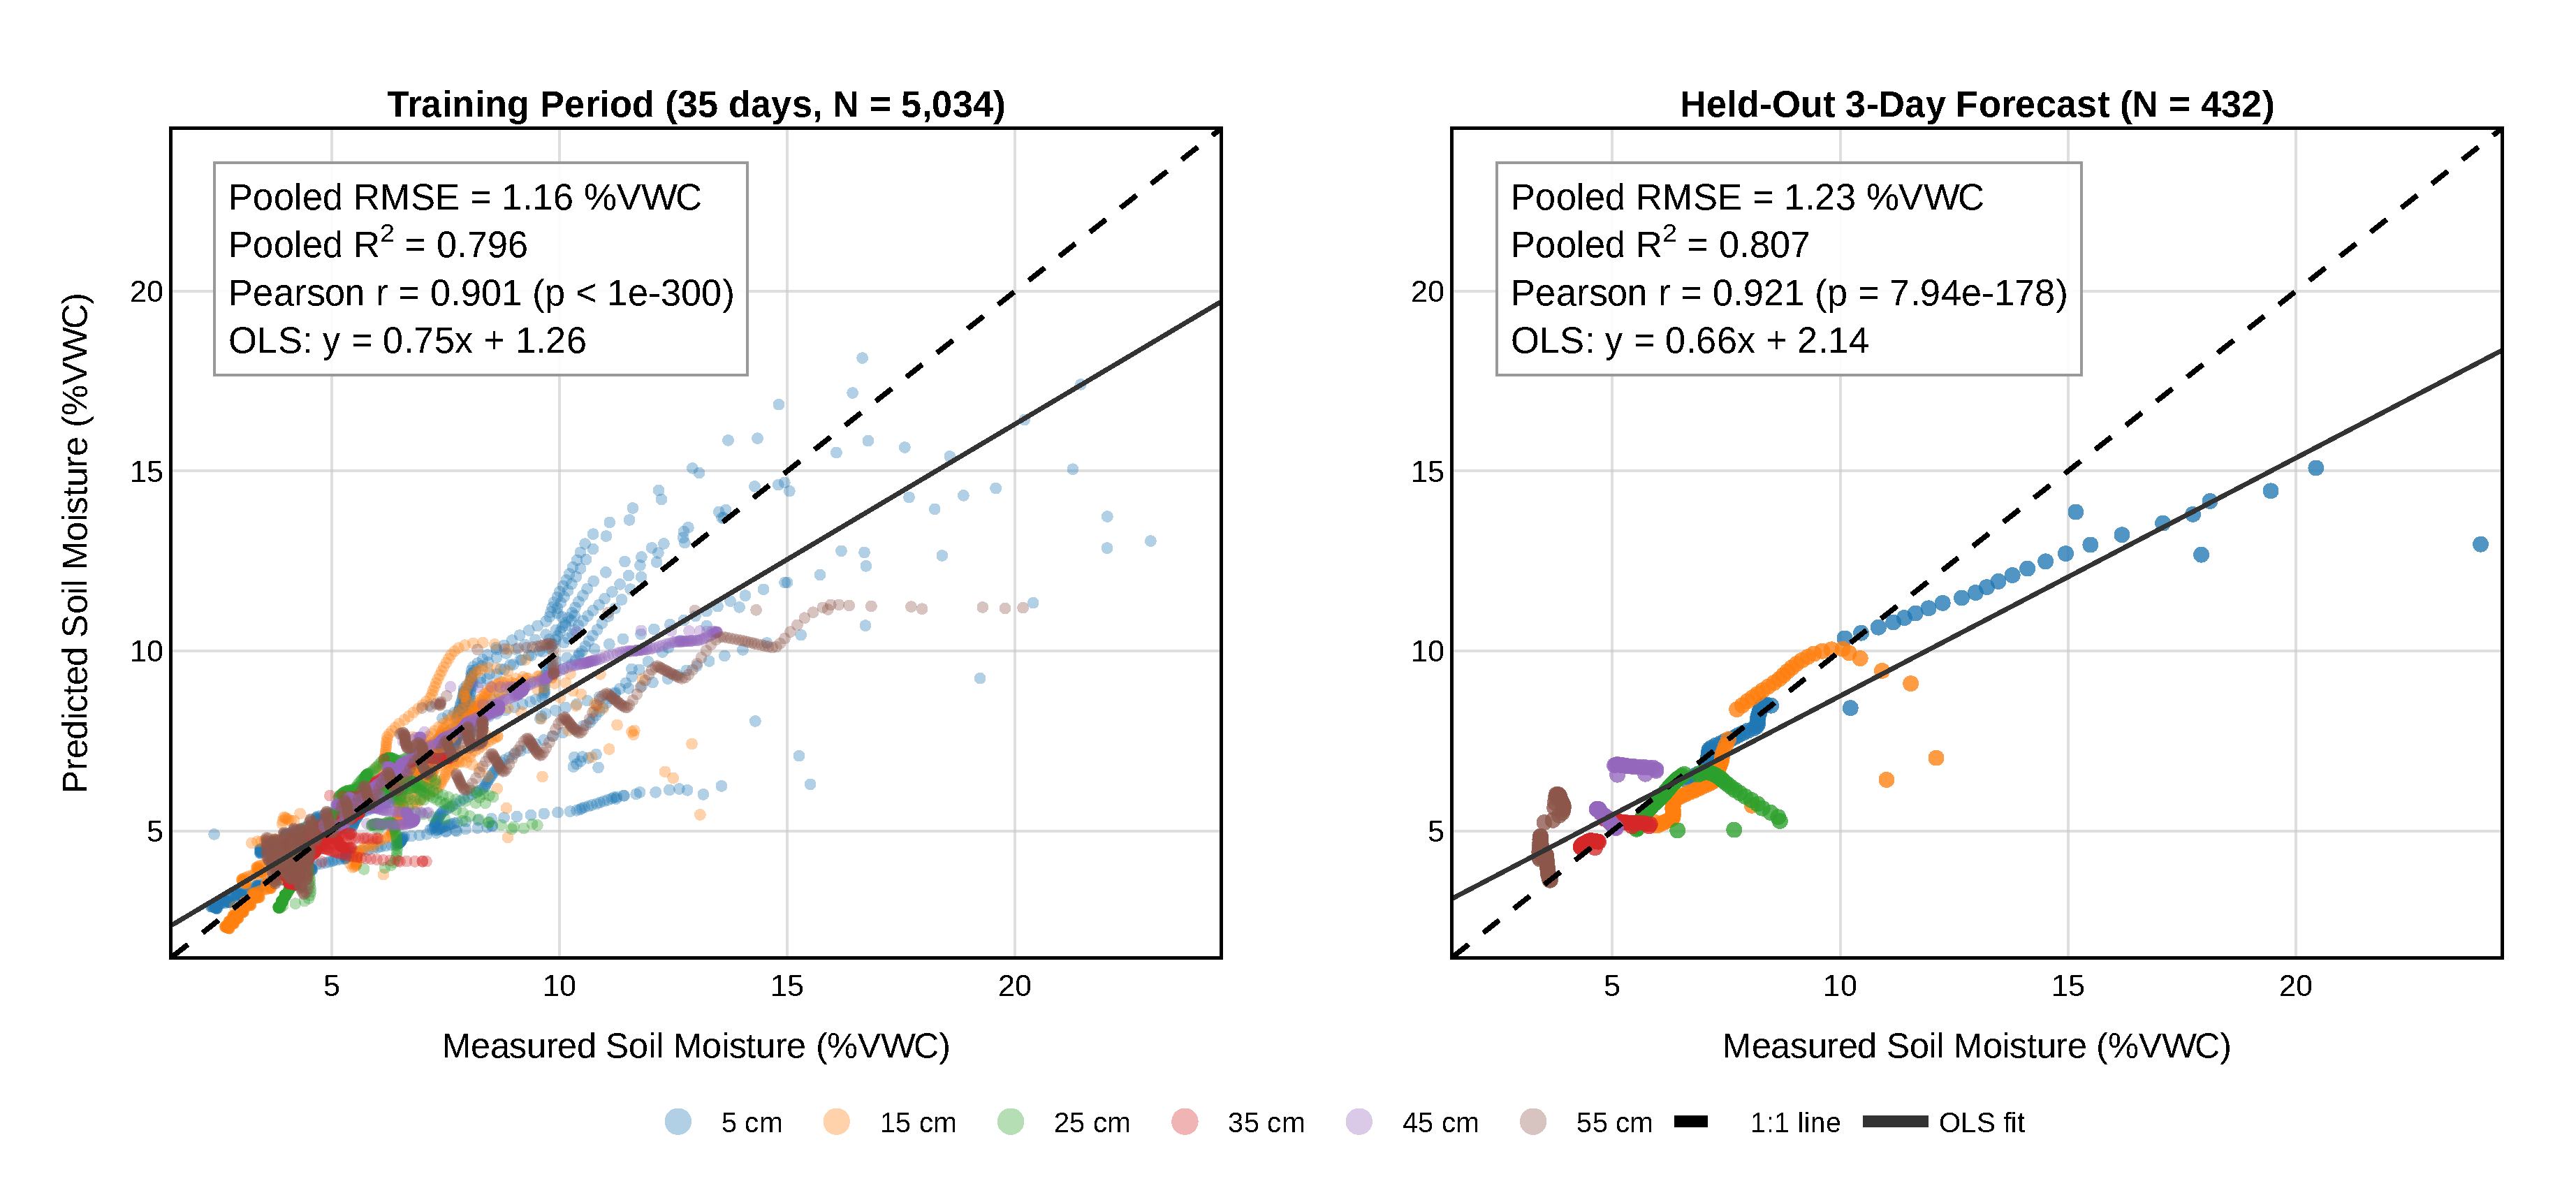
\includegraphics[width=0.96\linewidth]{predicted_vs_measured_scatter.pdf}
\marginnote{R-1.3c, R-2.5}\caption{\textcolor{blue}{Predicted versus measured soil moisture scatterplots across all six sensor depths (5--55~\si{cm}) for the 35-day training period ($N = 5{,}034$ concatenated points) and the 3-day held-out forecast ($N = 432$ points), showing tight clustering around the 1:1 line for low-variance deep layers (45--55~\si{cm}) alongside the profile-wide vertical span underlying the overall $R^2 = 0.807$ and $r = 0.921$.}}
\label{fig:scatter_parity}
\end{figure}

\begin{figure}[!htbp]
    \centering
    \includegraphics[width=\linewidth]{pinn_functions_vertical_by_layer.pdf}
    \marginnote{R-1.7, R-1.10, R-2.12}\caption{\textcolor{blue}{Estimated flux branches describing soil-water dynamics across sensor depths (5--55~\si{cm}, labeled along the left margin; formal branch definitions in Section~\ref{sec2}): $fr_i(r)$ is direct rainfall infiltration (\si{\%VWC/h}); $f_i(m_i)$ is gravitational vertical outflow (\si{\%VWC/h}); $f_{i,i+1}(m_i,m_{i+1})$ is signed potential-driven inter-layer exchange (\si{\%VWC/h}); $S_i(m_i,ET_0)$ is evapotranspirative depletion (\si{\%VWC/h}); $fl_i(m_i)$ is lateral ditch outflow (\si{\%VWC/h}, with scientific y-axis notation for compactness); and $fq_{\mathrm{irr}}(q_{\mathrm{irr}})$ is surface sprinkler inflow (\si{\%VWC/h}). Light blue regions denote the measured training moisture bounds at each depth.}}
    \label{estimatedflows}
\end{figure}

The most relevant result is that the PINN approach offers interpretable information for control design or direct decision-making. Fig.~\ref{estimatedflows} illustrates the estimated functions of measurable variables describing the soil water dynamics, such as rain, soil moisture, $ET_0$, and irrigation. These estimated flows constitute the PINN as differential equations that accomplish water balances at each soil layer \textcolor{blue}{(Section~\ref{sec2})}.
In the estimated functions, it is possible to observe that at the upper layer (5 \si{cm}), there is a linear relation between rain and soil moisture, where 30 \si{mm/h} of rain can induce an increase of 6 \si{\%VWC/h} in the soil moisture, and that in the third layer the direct increase is only 0.4 \si{\%VWC/h}. Moreover, it is observed that in the upper layer, 40 \si{\%VWC} induces vertical water movement that changes soil moisture by 3 \si{\%VWC/h}.

Furthermore, the estimated water movement associated with the potential difference between two soil layers is interlayer flow, ranging from -6 \si{\% VWC/h} (dark blue, upstream) to 3 \si{\%VWC/h} (yellow, downstream). It is noted that flows are generally consistent with potential gradients but are often negligible, consistent with sandy soil hydraulic properties \cite{Reyes2016}. The observed hydraulic trends between layers 1 and 2 can be attributed to changes in the soil induced by organic matter and agricultural practices.
The estimated \marginnote{R-2.6}\textcolor{blue}{evapotranspirative depletion} as a function of soil moisture and $ET_0$ increases with both. It is highlighted that layer 3 \textcolor{blue}{(25 \si{cm})} shows the maximum potential \textcolor{blue}{within the upper root zone} to produce high \textcolor{blue}{moisture extraction}, where at maxima of $ET_0$ and soil moisture, the produced change in soil moisture can be around 0.8 \si{\%VWC/h}, corroborating the proposed PINN as a tool to estimate soil regions where water must be guaranteed.
The estimated lateral outflow does not appear to be relevant for direct comparisons with the vertical movement of water. A particular small negative, non-monotonic behavior (despite the included constraints) appears in layer 5 and \marginnote{R-1.4, R-2.8}\textcolor{blue}{reflects both} lateral inflows from an adjacent ditch \textcolor{blue}{during storm surges and the fact that the physical penalties act as finite soft regularizers rather than hard algebraic barriers (Section~\ref{subsec2})}.
Finally, it is estimated how irrigation increases the soil moisture. In this case, irrigation is considered in the surface layer because the field used sprinkler irrigation; however, the PINN configuration can be adjusted to the selected irrigation system by setting this inflow to the layer where it is applied. The estimated function is predominantly linear, where soil moisture in the surface layer increases by approximately 5 \si{\%VWC/h} per hour of irrigation. This is crucial for control and decision-making processes. For instance, this curve enables us to quickly determine the irrigation required to bring a crop from a measured soil moisture level to a desired point that ensures adequate water uptake in the surface layers, which is crucial during the early stages of perennial crops.
The shaded blue regions highlight the span of measured soil moisture data used for training, making evident the benefits and effects of the \marginnote{R-2.7, R-2.8}\textcolor{blue}{soft physical regularizers} in the formulated approach, where, from sparse data, some functions like the vertical flow and lateral flow are reconstructed from the origin to far values following the positivity, monotonicity, and zero\textcolor{blue}{-forcing zero-flow regularizers.}

{\color{blue}\subsection{Ablation Study and Baseline Comparison}\label{sec:benchmarks}\marginnote{E-1.1, R-1.3d, R-2.10}

To verify each component of the proposed PINN and assess simpler or unconstrained alternatives, we evaluated seven configurations via free-run RK4 simulation ($\Delta t = \SI{1}{h}$) in Table~\ref{tab:benchmarks_master}. Forecasting accuracy is reported on the 35-day training period, the held-out 3-day test window, and 30 consecutive 3-day unseen test windows (obtained by sliding the 72-h forecast start forward one day at a time across May~3--June~5, 2025, each initialized from that day's measured $m(0)$). To test physical consistency directly, automatic differentiation was used to evaluate the partial derivatives of each layer's moisture rate $\dot{m}_i$ with respect to irrigation, rainfall, and $ET_0$ across all unseen operating points ($792\,\mathrm{h} \times 6\text{ layers} = 4{,}752$ evaluations), recording the percentage of states that violate basic hydrology---namely, irrigation drying the soil ($\partial \dot{m}/\partial q_{\mathrm{irr}} < 0$), rainfall drying the soil ($\partial \dot{m}/\partial r < 0$), or evaporative demand wetting the soil ($\partial \dot{m}/\partial ET_0 > 0$).

\begin{table}[!htbp]
\centering
\marginnote{E-1.1, R-1.3d, R-2.10}\caption{Ablation and baseline comparison pairing free-run forecasting RMSE (\si{\%VWC}) with unphysical input-derivative rates across unseen field states ($792\,\mathrm{h} \times 6$ layers) and flux/depletion interpretability.}
\label{tab:benchmarks_master}
\fontsize{6.3}{8.0}\selectfont
\setlength{\tabcolsep}{1.0pt}
\begin{tabular*}{\textwidth}{@{\extracolsep{\fill}}lccccccc@{}}
\toprule
 & \multicolumn{3}{c}{Free-Run RMSE (\si{\%VWC})} & \multicolumn{3}{c}{Unphysical Derivative Rate (\%)} & Flux \& \\
\cmidrule(lr){2-4}\cmidrule(lr){5-7}
Model & 35-d Train & 3-d Test & 30 Unseen 3-d & $\frac{\partial \dot{m}}{\partial q_{\mathrm{irr}}}{<}0$ & $\frac{\partial \dot{m}}{\partial r}{<}0$ & $\frac{\partial \dot{m}}{\partial ET_0}{>}0$ & Depletion \\
 & RMSE ($R^2$) & RMSE ($R^2$) & Mean$\pm$SD & (dries) & (dries) & (wets) & Curves? \\
\midrule
\multicolumn{8}{@{}l}{\textit{A. Proposed PINN and architectural ablations}} \\[1pt]
\textbf{Proposed PINN (Full)} & \textbf{1.16 (0.80)} & \textbf{1.23 (0.81)} & \textbf{1.04$\pm$0.53} & \textbf{0.0} & \textbf{0.0} & \textbf{2.5}$^\dagger$ & \textbf{Yes} \\
Ablation 1 (Stage 1 only) & 2.52 (0.03) & 1.55 (0.70) & 1.33$\pm$0.35 & 0.0 & 0.0 & 1.0 & Yes \\
Ablation 2 (Unregularized) & 1.48 (0.67) & 1.39 (0.76) & 1.00$\pm$0.30 & 0.0 & 33.0 & 42.0 & Violated$^\ddagger$ \\
\midrule
\multicolumn{8}{@{}l}{\textit{B. Reference baselines (uninterpretable or physically unconstrained)}} \\[1pt]
Persistence ($\dot{m}=0$) & 2.44 (0.09) & 1.91 (0.54) & 1.86$\pm$1.02 & --- & --- & --- & No \\
Linear State-Space ODE & 1.35 (0.72) & 0.97 (0.88) & 0.82$\pm$0.27 & 33.3 & 0.0 & 33.3 & No \\
Black-Box ODE (374k) & 0.91 (0.87) & 1.13 (0.84) & 0.98$\pm$0.57 & 70.5 (52.9$^*$) & 32.6 & 40.7 & No \\
Black-Box ODE (2.2k) & 0.85 (0.89) & 1.26 (0.80) & 1.77$\pm$2.43 & 73.4 (96.8$^*$) & 20.7 & 28.2 & No \\
\bottomrule
\end{tabular*}
\begin{tablenotes}
\footnotesize
\item $^*$In the 5-\si{cm} topsoil layer alone, $\partial \dot{m}_1/\partial q_{\mathrm{irr}} < 0$ occurs on 52.9\% (Black-Box 374k) and 96.8\% (Black-Box 2.2k) of unseen hours.
\item $^\dagger$Residual from soft-penalty training convergence near dry states ($\le +0.01\,\si{\%VWC/h}$), negligible relative to sensor resolution.
\item $^\ddagger$Without physical regularizers, 26.7\% of learned branch evaluations become negative and 19.5\% violate monotonicity.
\end{tablenotes}
\end{table}

Both ablations confirm the design in Section~\ref{Methodology}: omitting Stage-2 trajectory refinement (\textbf{Ablation~1}) raises 3-day RMSE from 1.23 to 1.55~\si{\%VWC} (training: 1.16 to 2.52~\si{\%VWC}) due to integration drift, whereas removing the physical regularizers (\textbf{Ablation~2}) raises 3-day RMSE to 1.39~\si{\%VWC} and introduces 33.0\% rain and 42.0\% $ET_0$ sign violations, while the full PINN reduces 3-day error by 35.6\% over \textbf{Persistence} (1.91 to 1.23~\si{\%VWC}; 53.2\% in the 5-\si{cm} topsoil, from 4.32 to 2.02~\si{\%VWC}). In the full PINN, the small 2.5\% residual on $\partial \dot{m}/\partial ET_0 > 0$ simply reflects soft-penalty convergence near dry states, with negligible magnitude ($\le +0.01\,\si{\%VWC/h}$ vs.\ $+1.22$ to $+2.22\,\si{\%VWC/h}$ in black-box models). Crucially, although unconstrained \textbf{Linear ODE} ($\dot{m} = Am + Bu + c_0$) and two-stage \textbf{Black-Box ODE} ($\dot{m} = \mathrm{MLP}(m, q_{\mathrm{irr}}, r, ET_0)$) reach slightly lower passive 3-day RMSE (by 0.10--0.26~\si{\%VWC}), this stems from sparse field data dominated by routine wetting pulses: rain and fixed 2-hour sprinkler runs ($q_{\mathrm{irr}} \in \{0, 0.5, 1.0\}\,\si{h/h}$) account for 96.2\% of hourly $\Delta m$ variance, whereas slow daytime $ET_0$ drying accounts for only 1.6\%. Fitting historical cases alone causes unconstrained models to invert physical responses across 20.7\%--73.4\% of unseen states---predicting soil drying under shorter irrigation doses (6--15~\si{min}) and root-zone wetting under high $ET_0$, with no flux or depletion curves. In real agricultural systems, where field measurements are sparse and uncontemplated weather or management conditions frequently arise, statistical case-fitting alone is insufficient; embedding governing physics as prior information is essential for reliable decision-making and control.

\subsection{Agronomic and Hydrological Interpretation}\label{sec:uptake_rationale}

In\marginnote{R-1.3d, R-1.4, R-2.6} Figs.~\ref{Mainfig} and~\ref{estimatedflows}, the PINN estimates daytime moisture loss using only soil moisture and $ET_0$, without direct plant sensors. Because surface evaporation, root water uptake, and ditch evaporation all follow the daily $ET_0$ cycle, these estimates reflect total $ET_0$-driven drying rather than plant transpiration alone. Across the raised bed (Fig.~\ref{fig:bed_ditch}), this drying separates naturally by depth: surface evaporation and shallow uptake at 5~\si{cm} ($\approx\SI{0.22}{mm/d}$), active root-zone uptake at 15--25~\si{cm} that peaks at 25~\si{cm} ($\approx\SI{0.28}{mm/d}$) just above the $\approx\SI{30}{cm}$ clay layer, minimal loss inside the 35--45~\si{cm} clay layer ($\approx\SI{0.05}{}$--$\SI{0.11}{mm/d}$), and daytime water-table drawdown toward the adjacent ditch at 55~\si{cm} ($\approx\SI{1.30}{mm/d}$).

Summed\marginnote{R-1.3d, R-2.6} over 24-h cycles, total profile drying averages $\approx\SI{2.04}{mm/d}$ in training and $\approx\SI{1.89}{mm/d}$ in the unseen period ($\approx\SI{0.58}{mm/d}$ within 0--30~\si{cm}), matching spring evapotranspiration reported for Florida citrus ($2$--$\SI{5}{mm/d}$)~\cite{Morgan2006, Kadyampakeni2014}. The peak at 25~\si{cm} also agrees with Florida citrus field studies showing that 64\%--90\% of fibrous feeder roots concentrate in the top 30~\si{cm}---particularly within the top $\sim\SI{25}{cm}$ (\SI{10}{in}) wetted by microsprinklers above shallow Flatwoods clay horizons~\cite{Morgan2006, Morgan2007, Castle1993, Kadyampakeni2014, Johnson2023}. Even so, active root depth is not constant: differences in soil horizons, bed geometry, irrigation schedules, fertilization, and HLB root loss can shift where trees extract water~\cite{Kadyampakeni2014, Kwakye2023, Johnson2023}. Because weighing lysimeters or root coring are impractical in commercial groves, whereas soil moisture probes are affordable and widely adopted, estimating uptake zones from probe data offers a practical way to guide smart irrigation controllers.

To\marginnote{R-1.3a, R-2.11} evaluate what this means for water management, we compared free-run PINN simulations with and without the grower's routine 2--3~\si{h} sprinkler runs ($\approx\SI{4.7}{mm}$ per hour of irrigation, totaling $\approx\SI{85.1}{mm}$ in training and $\approx\SI{79.7}{mm}$ in the unseen period). Under this fixed schedule, $11\%$--$17\%$ ($\approx\SI{9.4}{}$--$\SI{13.7}{mm}$) of the applied irrigation water drains by gravity below 30~\si{cm} ($\sim 8\%$ net downward loss after partial upward capillary return), moving past the main root zone. Furthermore, two 2-\si{h} runs ($\approx\SI{18.8}{mm}$, or $24\%$ of unseen-period irrigation) occurred less than 24~\si{h} before heavy rainstorms (18.5 and \SI{9.1}{mm}). While field control trials remain future work, these results indicate that combining the PINN with weather forecasts in an MPC controller---keeping wetting fronts above 30~\si{cm} and skipping pre-storm irrigations---could reduce deep percolation and nutrient leaching~\cite{Morgan2006, Obreza2010}.}

{\color{blue}\subsection{Conclusions}\marginnote{E-1.1, R-2.11}
Accurate forecasting of multi-depth soil moisture dynamics has been constrained by analytical Richards' equation solvers requiring intensive site-specific hydraulic calibration and by unconstrained black-box models that lack physical consistency for predictive control. Here, we show that embedding a sensor-depth discretization of Richards' equation into a physically regularized two-stage PINN reconciles flux-level interpretability with operational multi-day forecasting accuracy.

Validated\marginnote{E-1.1, R-1.3a, R-1.3d, R-2.10} on field telemetry from a commercial raised-bed Florida citrus block, the proposed PINN predicts hourly soil moisture across six depths (5--55~\si{cm}) over a 3-day held-out horizon with an overall RMSE of \SI{1.23}{\%VWC} ($\approx\SI{3.22}{mm}$ equivalent profile variation, $R^2 = 0.807$, Pearson $r = 0.921$), reduces 3-day error by 35.6\% relative to persistence, outperforms single-stage and unregularized ablations, and avoids the physically reversed actuation responses exhibited by unconstrained baselines while exposing explicit irrigation gain and evapotranspirative depletion curves.

Three\marginnote{E-1.1, R-2.3, R-2.11} scope boundaries merit emphasis: (i) calibration and validation reflect a single raised-bed sandy Alfisol citrus site over a 35-day training and 33-day spring unseen dataset driven by observed station meteorology, so generalization to finer-textured soils, other crops, and live numerical weather forecasts requires multi-site, multi-season testing; (ii) hourly sampling matched to forecast providers smooths sub-hourly infiltration peaks in sandy topsoil; and (iii) while the PINN satisfies structural and Jacobian conditions suitable for MPC, closed-loop field MPC deployment and direct measurement of irrigation water savings remain future work.}

\section{Methodology: PINN Formulation} \label{Methodology}
\subsection{Problem Statement}
We address the formulation of a model suitable for precise decision-making in irrigation management. The model's precision is primarily focused on vertical water distribution, where, in a horizontally homogeneous soil region, soil moisture measurements from a particular section can be considered significant for making informed irrigation decisions. This practice is common in most commercial settings where irrigation is managed using soil moisture sensors \cite{Rossini2021, Mandal2025}.
Therefore, the model must accurately describe the vertical dynamics of soil moisture and their interaction with \marginnote{R-1.2, R-1.10, R-2.6}\textcolor{blue}{evapotranspirative plant-soil sink processes}, environmental variables, and irrigation. Specifically, the model must describe the soil moisture dynamics at the targeted measured soil layers $m_i(t)$ \textcolor{blue}{(\si{\%VWC})}. 
Moreover, at each layer, the model must explain the effects of measurable external inputs, such as rainfall $r(t)$ (\si{mm/h}), irrigation rate \textcolor{blue}{$q_{\mathrm{irr}}(t)$} (\si{h/h}), and potential evapotranspiration \textcolor{blue}{$ET_0(t)$} (\si{mm/h}), which \textcolor{blue}{drives root-zone water depletion}.
In addition, the model must be interpretable, physically consistent, and stable, mirroring the stability observed in the real system under unsaturated conditions.
Importantly, the model must allow the incorporation of valuable forecast information in its numerical simulation over extended horizons to support the formulation of model predictive control (MPC) frameworks.


\subsection{Proposed Approach}

Figure \ref{diagramalgorithm} describes the proposed PINN architecture and training process. The architecture comprises an input layer associated with variables that can be obtained from field sensors, estimated, or obtained from forecasting services; therefore, the measured soil moisture initial condition ($m(0)$), measured irrigation, measured evapotranspiration, measured rainfall, and the current estimated soil moisture ($\hat{m}(t)$) are considered as inputs.

The hidden layers are designed to match the structure of a spatially discretized Richards' equation, with $n$ vertical layers corresponding to the depths of installed soil moisture sensors in the field. These layers are configured as fluxes that are functions of the measured and estimated variables. These fluxes represent elements of Richards' equation, such as gravitational drainage and capillary-driven water movement. Moreover, these fluxes include inflow from rainfall and irrigation and incorporate plant water uptake as a function of $ET_0$ and soil moisture. Therefore, the fluxes in the hidden layers are modeled by neural networks with parameters $\Theta$ that form the dynamic model, a set of differential equations describing the temporal variation of soil moisture in each layer. This set of differential equations is numerically solved using a 4th-order Runge–Kutta (RK4) algorithm, which is integrated directly into the training and implementation routines.

The training process searches for the $\Theta$ parameters that promote an accurate description of the SM dynamics of the real system. The training process utilizes recorded windows of training data. The integration of the RK4 routine into the training process ensures a solution that, starting from a measured initial soil moisture condition $m(0)$, uses rainfall, potential evapotranspiration, and irrigation data to provide an optimal or near-optimal description of soil moisture dynamics. This inclusion contributes to model stability and generality. However, including numerical integration of the model in the training process significantly complicates the optimization problem. Therefore, the training is conducted in two stages. The first stage minimizes the derivative losses between measured and estimated soil moisture variations; this routine does not require numerical integration and is a strategy for finding a point to initialize the $\Theta$ parameters near a feasible solution. The second stage employs the tracking loss, which embeds the model's numerical solution to align the estimated SM ($\hat{m}(t)$) with the measured SM ($m(t)$).
Furthermore, the cost function incorporates three penalization conditions: positivity ensures the correct flow direction in the discretized Richards' equation, monotonicity guarantees flow correlation with driving variables, and zero-potential zero-flux enforces the absence of flow when no water source is present.
Ultimately, a trained model with its respective numerical solver is obtained. This model allows the inclusion of external inputs, such as rainfall and $ET_0$, which can be obtained directly or inferred from forecasting services. Importantly, the model is also a function of the irrigation (the control input), which can be obtained using predictive control approaches or used to evaluate multiple irrigation scenarios. Moreover, including water uptake, treated as a function of $ET_0$ and soil moisture, in the overall model enables inference of the amount of water correlated with plant water uptake, helping dynamically identify and prioritize regions where the estimated plant is absorbing the most water.
Subsequently, a detailed description of the model's modeling, formulation, training, and implementation in a real citrus field is provided.

\begin{figure}[!htbp]
		\centering
		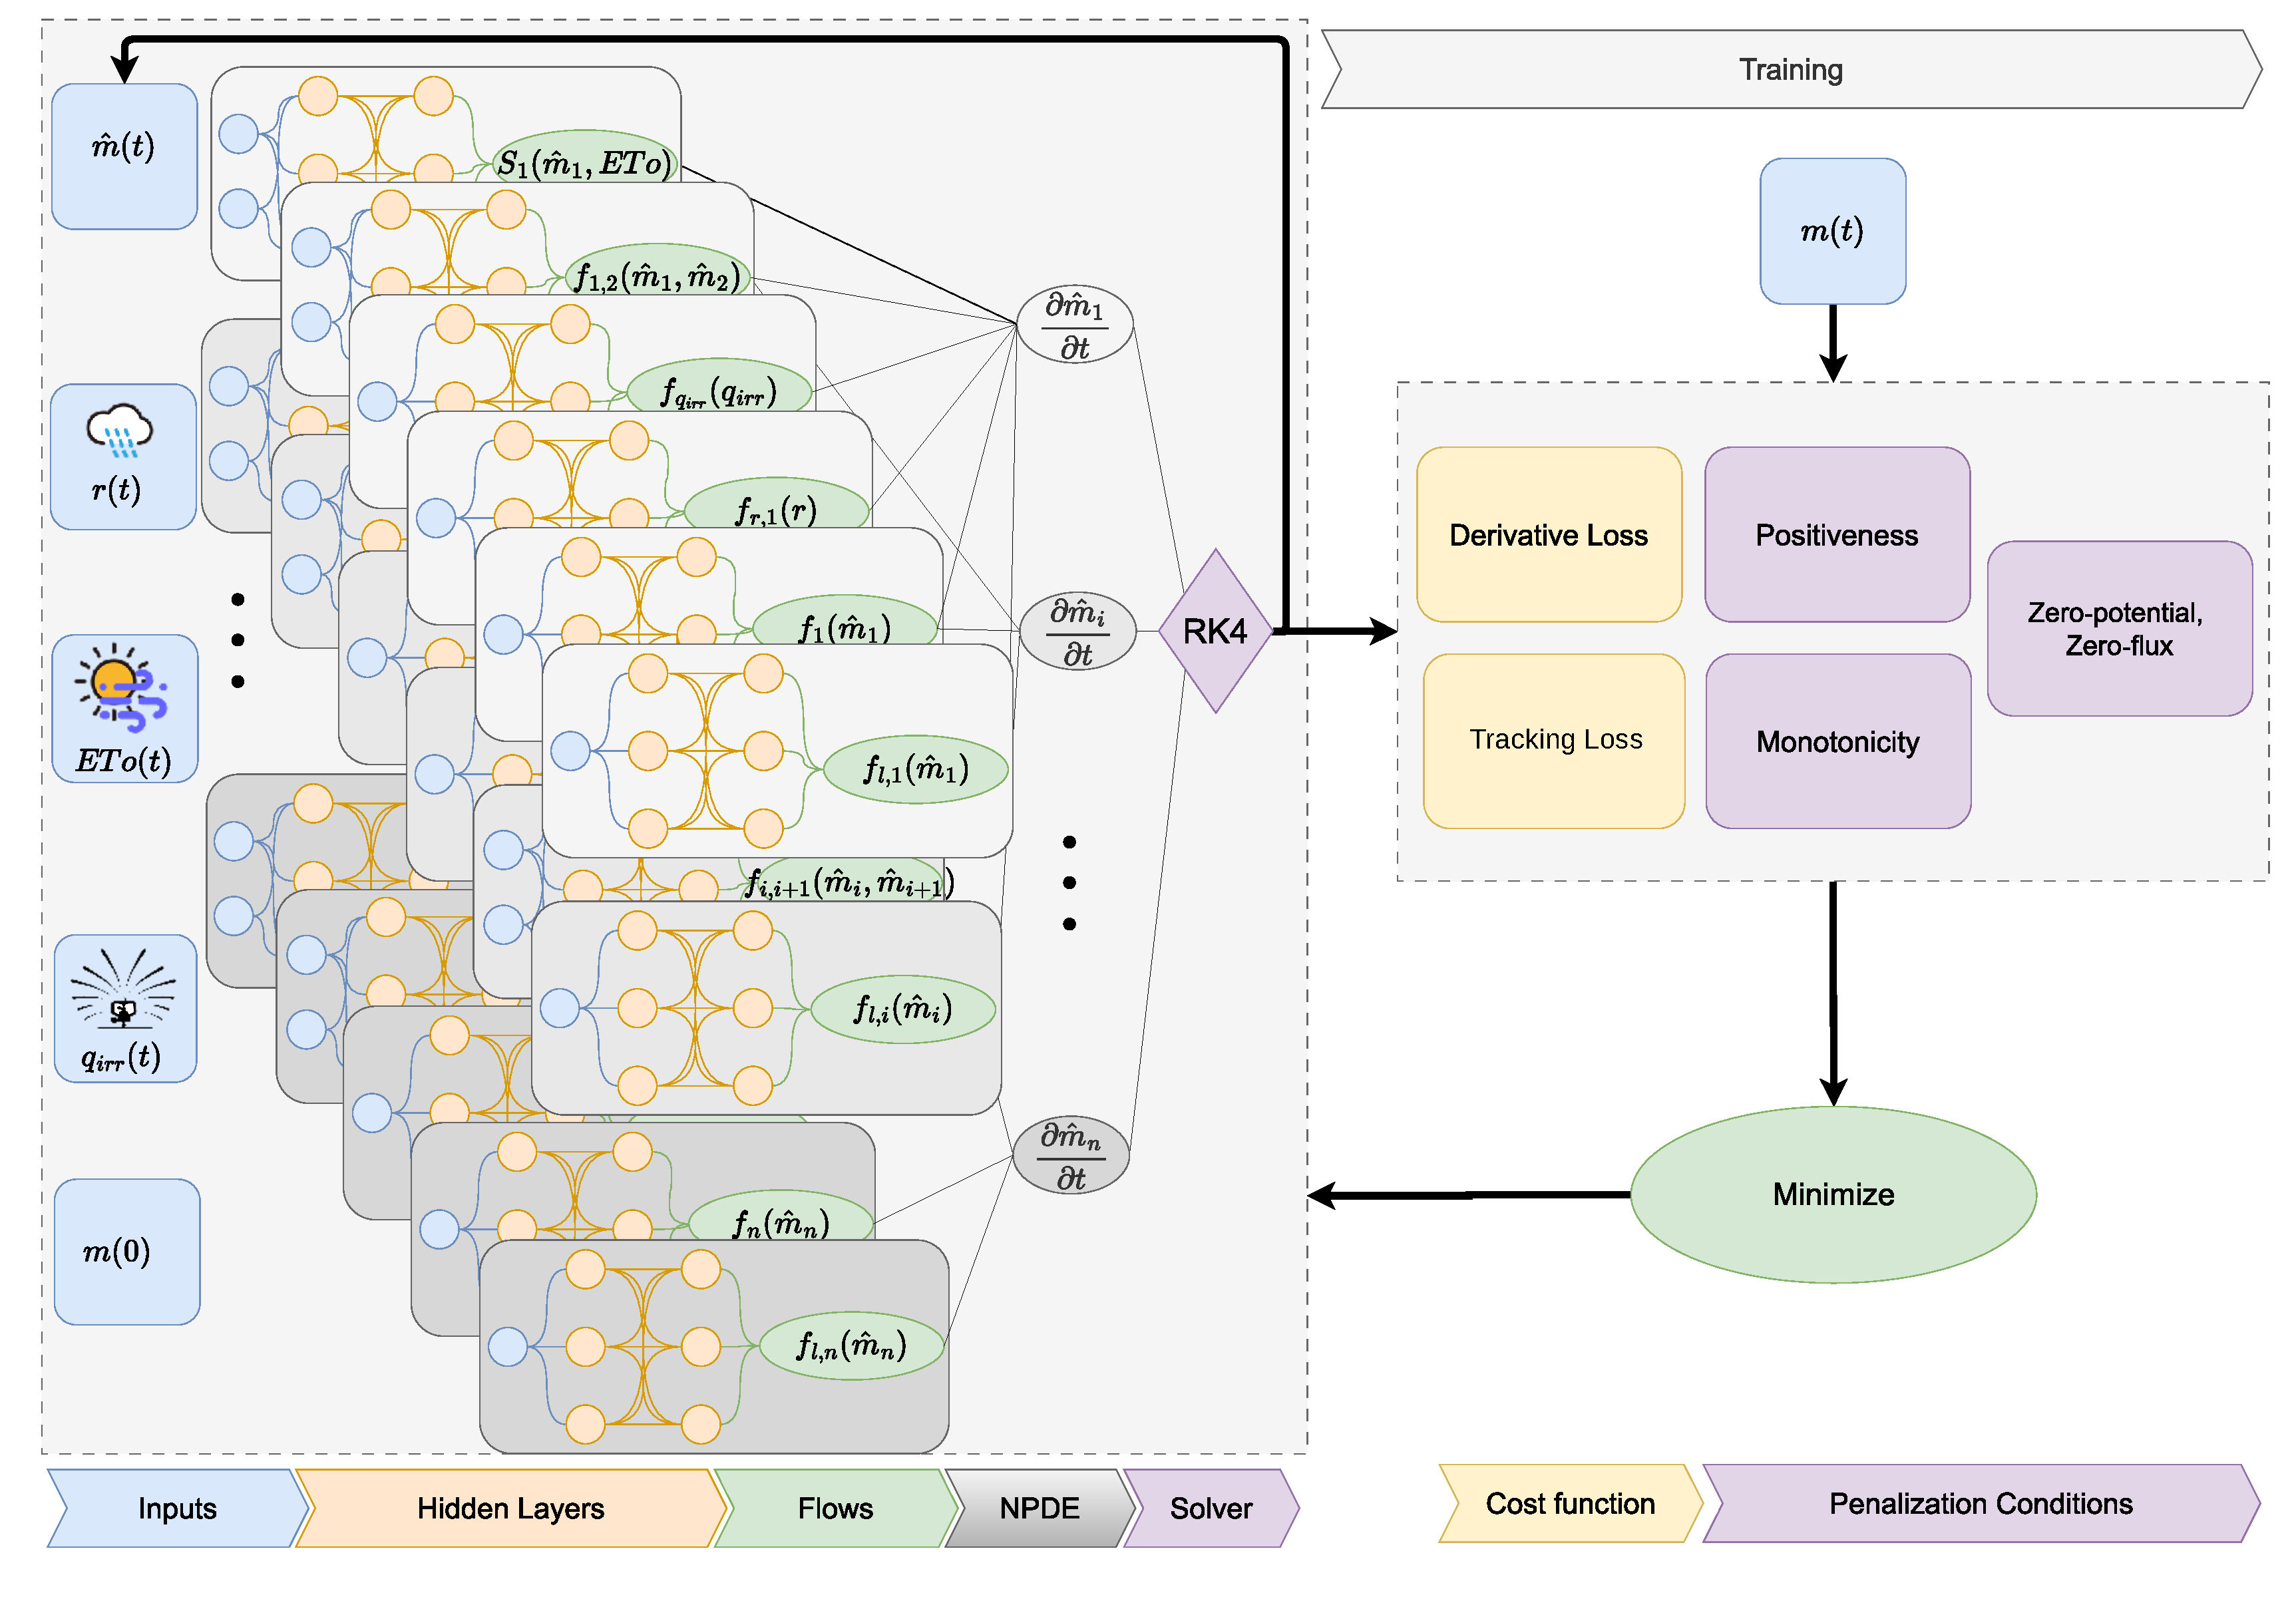
\includegraphics[width=0.92\textwidth]{PINNsmb.pdf}
		\marginnote{R-1.6, R-1.10, R-2.12}\caption{\textcolor{blue}{Architecture and two-stage training workflow of the proposed PINN. Inputs comprise the 6-layer moisture vector $\hat{m}(t)$ (5--55~\si{cm}), irrigation ($q_{\mathrm{irr}}$), rainfall ($r$), and reference evapotranspiration ($ET_0$). Inside $g(\hat{m},r,ET_0,q_{\mathrm{irr}},\boldsymbol{\Theta})$, neural branches model vertical drainage $f_i(m_i)$, signed inter-layer exchange $f_{i,i+1}(m_i,m_{i+1})$ ($i=1\dots5$), lateral ditch outflow $fl_i(m_i)$ ($i=1\dots5$; $f_6$ captures lower boundary discharge), rainfall infiltration $fr_i(r)$, surface irrigation $fq_{\mathrm{irr}}(q_{\mathrm{irr}})$, and evapotranspirative sink $S_i(m_i,ET_0)$ ($pc_i$). Stage~1 minimizes derivative loss $j_1$ and Stage~2 refines $\boldsymbol{\Theta}$ via RK4 trajectory tracking loss $j_2$, subject to soft penalties $c_1$--$c_3$.}}
		\label{diagramalgorithm}
  \vspace{-1em}
\end{figure}

\subsubsection{Model}\label{sec2}

The developed Physics-Informed Neural Network (PINN) is formulated using a spatial discretization of Richards' equation, which describes vertical water movement in the soil as a function of soil moisture. We propose a spatial discretization by dividing the soil into $n$ layers, with each layer associated with available soil moisture measurements. The objective is to determine the rate of change of soil moisture in each layer due to gravity and water potential. \marginnote{R-2.2}\textcolor{blue}{For downward-positive depth $z$ and total hydraulic head $H = h(m) - z$, Richards' equation is:}
\begin{equation}
\frac{\partial m}{\partial t} = \frac{\partial }{\partial z}\left[ K(m)\left(\frac{\partial h(m)}{\partial z} \textcolor{blue}{-} 1\right)\right]\textcolor{blue}{,}
\label{Richards}
\end{equation}
\textcolor{blue}{where} $m$ is the soil moisture, $z$ is the vertical axis, considered to increase downward, $K(m)$ is the hydraulic conductivity, which depends on soil moisture, and $h(m)$ is the soil-water pressure head.

The Richards' equation obeys the continuity relation; thus, by defining $q$ as a \textcolor{blue}{downward} water flux, the continuity relation is given by:
\begin{equation}
\frac{\partial m}{\partial t} = -\frac{\partial q}{\partial z}\textcolor{blue}{.}
\label{continuity}
\end{equation}

Therefore, from Eq.~\textcolor{blue}{\eqref{Richards}} and Eq.~\textcolor{blue}{\eqref{continuity}}, the Darcy--Buckingham law can be extracted as:
\begin{equation}
q = \textcolor{blue}{-K(m)\frac{\partial H}{\partial z} =} K(m)\left(\textcolor{blue}{1 - \frac{\partial h(m)}{\partial z}}\right)\textcolor{blue}{.}
\label{eq:darcy}
\end{equation}
If a spatial discretization along $z$ with a fixed spatial step $\Delta z$ is proposed, \textcolor{blue}{evaluating $-\partial h/\partial z \approx (h(m_i)-h(m_{i+1}))/\Delta z$ across the interface between layers $i$ and $i+1$,} the flux $q_i$ leaving layer $i$ downwards to the layer $i+1$ is given by:
\begin{equation}
q_i = K(m_i)\left(\frac{h(m_i)-h(m_{i+1})}{\Delta z}+1\right)\textcolor{blue}{.}
\label{eq:flux_disc}
\end{equation}
Similarly, the continuity equation describing moisture conservation in a layer $i$ can be discretized as:
\begin{equation}
\frac{d m_i}{d t} = \frac{q_{i-1}(t)-q_i(t)}{\Delta z}.
\label{eq:cont_disc}
\end{equation}
\textcolor{blue}{At the column boundaries, the surface layer ($i=1$) receives rainfall and sprinkler irrigation minus surface evaporative losses, while the bottom boundary ($i=n$, \SI{60}{cm}) discharges vertically via $f_n(m_n)$.}

Therefore, a discretized description of soil water dynamics at a layer $i$ is provided by
\begin{equation}
\begin{aligned}
\frac{d m_i}{d t} &= K(m_{i-1})\left(\frac{h(m_{i-1})-h(m_{i})}{\Delta z^2}\right) + \frac{K(m_{i-1})}{\Delta z} \\
&\quad - K(m_{i})\left(\frac{h(m_{i})-h(m_{i+1})}{\Delta z^2}\right) - \frac{K(m_{i})}{\Delta z}.
\end{aligned}
\label{eq:disc_richards}
\end{equation}

From this discretized formulation, it can be observed that the rate of change of soil moisture at each $i$-th layer, driven by gravity and potential forces, can be described as functions (to be estimated) of measured soil moisture in the respective and adjacent layers. Specifically, we are proposing a structure where
\begin{equation}
\begin{aligned}
K(m_{i})\left(\frac{h(m_{i})-h(m_{i+1})}{\Delta z^2}\right) &\approx f_{i,i+1}({m}_i,{m}_{i+1}), \\ 
\frac{K(m_{i})}{\Delta z} &\approx f_i({m}_i)\textcolor{blue}{,}
\end{aligned}
\end{equation}
\textcolor{blue}{where $f_i(m_i) \ge 0$ represents downward gravitational drainage and $f_{i,i+1}(m_i, m_{i+1})$ represents signed potential-driven exchange (positive downward when $m_i > m_{i+1}$ and negative upward for capillary rise when $m_{i+1} > m_i$).\marginnote{R-2.2, R-2.8}}

Moreover, additional functions describing the rate of change produced by actions such as irrigation, rainfall, water uptake, and horizontal water movement can be incorporated to obtain a model structure that could be useful for evaluating how soil moisture dynamics evolve over time in response to external variables. Specifically, \textcolor{blue}{$q_{\mathrm{irr}}$} is incorporated as the irrigation related variable, and \textcolor{blue}{$fq_{\mathrm{irr}}(q_{\mathrm{irr}})$} is a function that explains the rate of change of the soil moisture in relation to irrigation\textcolor{blue}{;}\marginnote{R-1.5, R-1.10} note that \textcolor{blue}{$q_{\mathrm{irr}}$} could have units of flow (e.g., \si{m\textcolor{blue}{^3}/h}) or units of relative time (e.g., \si{h/h}) indicating how much irrigation was active during a period of time. In the first case, \textcolor{blue}{$fq_{\mathrm{irr}}(q_{\mathrm{irr}})$} provides a relation between applied flow and change in soil moisture, and in the second case, \textcolor{blue}{$fq_{\mathrm{irr}}(q_{\mathrm{irr}})$} provides a relation between duration of irrigation time and change in soil moisture. In this study, we assume that irrigation is applied only at the top, but its location can be accommodated depending on the irrigation system used, e.g., subsurface drip irrigation. 
The rainfall, $r$, is considered an input in \si{mm/h} and can be obtained from a weather station in the crop or from meteorological services, where predictions are also available. The function, $fr_i(r)$, accounts for the direct effect of rain at each soil layer. This is because crops are often planted in beds, allowing rain to wet exposed soil layers directly.

Furthermore, we incorporate a sink component to estimate soil moisture changes due to \marginnote{R-2.6}\textcolor{blue}{evapotranspirative depletion} in each layer, which is a key motivation for this study. This sink is represented by \textcolor{blue}{an evapotranspirative sink function}, $S_i (m_i, ET_0)$ \textcolor{blue}{(denoted $pc_i$ in Section~\ref{Results})}, describing \textcolor{blue}{moisture depletion} at each layer. This \textcolor{blue}{depletion} is determined by atmospheric, plant, and soil conditions \cite{swap2024}. Specifically, we propose that this \textcolor{blue}{sink} is a function of the available water at the respective layer ($m_i$) and the potential evapotranspiration ($ET_0$).

Additionally, we include an outlet lateral flow, $fl_i (\textcolor{blue}{m_i})$, associated with \marginnote{R-1.4}\textcolor{blue}{subsurface drainage toward adjacent ditches} when excess water prevents flow between layers. This is considered an outlet, as most crops are planted in raised beds between furrows \textcolor{blue}{or ditches} to facilitate drainage.

In summary, we are formulating a PINN to estimate the dynamics of a system with $n$ soil layers \marginnote{R-1.10, R-2.2}\textcolor{blue}{($n=6$)} as follows:
\begin{equation}
\label{system}
\begin{aligned}
\frac{d{m}_1}{dt} = & - f_1({m}_1) - f_{1,2}({m}_1,{m}_2) - fl_1(m_1) - S_1({m}_1, ET_0) + fr_1(r) + \textcolor{blue}{fq_{\mathrm{irr}}(q_{\mathrm{irr}})}\\
\frac{d{m}_i}{dt} = & f_{i-1}({m}_{i-1}) + f_{i-1,i}({m}_{i-1},{m}_i) - f_i({m}_i)- f_{i,i+1}({m}_i,{m}_{i+1}) - fl_i(\textcolor{blue}{m_i}) \\ 
 & - S_i({m}_i, \textcolor{blue}{ET_0}) + fr_i(r), \qquad \textcolor{blue}{i = 2,\dots,n-1,}\\
\frac{d{m}_n}{dt} = & f_{n-1}({m}_{n-1}) + f_{n-1,n}({m}_{n-1},{m}_n) - f_n({m}_n) - S_n({m}_n, \textcolor{blue}{ET_0}) + fr_n(r)\textcolor{blue}{.}
\end{aligned}
\end{equation}
Note that at layer $n$ \textcolor{blue}{($n=6$, \SI{55}{cm})}, we exclude the lateral flow term $fl_n$. In the upper layers, the vertical flow $f_i$ delivers water to the layer below, making it distinct from the lateral flow $fl_i$, which exits the system. However, at layer $n$, both $f_n$ and $fl_n$ would represent outflows that leave the soil column without feeding another layer, making them similar.

\subsubsection{PINN Structure}
In our approach, we use the system structure proposed in (Eq. \eqref{system}) to define the PINN structure. Therefore, as shown in Fig. \ref{diagramalgorithm}, we are proposing an NN with branches that emulate the functions \( g \in \{f_i, f_{i,i+1}, S_i, \marginnote{R-1.10}\textcolor{blue}{fq_{\mathrm{irr}}}, fr_i, fl_i\} \). Therefore, each branch is a Multilayer Perceptron (MLP) with depth \( L \) and width \( H \), given by
\begin{equation}
\phi\!\bigl(\mathbf{x}; \boldsymbol{\Theta}\bigr)
  =\;
  \mathbf{W}^{(L)}
  \,\mathcal{A}\!\Bigl(
     \mathbf{W}^{(L-1)}
     \,\mathcal{A}\!\bigl(
        \dots
        \,\mathcal{A}\!\bigl(
           \mathbf{W}^{(1)}\mathbf{x}
           +\mathbf{b}^{(1)}
        \bigr)
        +\mathbf{b}^{(L-1)}
     \bigr)
  \Bigr)
  +\mathbf{b}^{(L)},
\label{eq:mlp}
\end{equation}
where \(\mathcal{A}(\cdot)\) is the activation function, and \(\displaystyle \boldsymbol{\Theta} = \{\mathbf{W}^{(\ell)},\,\mathbf{b}^{(\ell)}\}_{\ell=1}^L\) is the set of trainable parameters. The input \(\mathbf{x}\) denotes the argument of each flux function.
In cases where the function depends on a single variable $\left(f_i(m_i),\;\textcolor{blue}{fq_{\mathrm{irr}}(q_{\mathrm{irr}}),\;fr_i(r),\;fl_i(m_i)}\right)$, we have \(\mathbf{x}\in\mathbb{R}\), and when the function depends on two variables \(f_{i,i+1}(m_i,m_{i+1})\), \(\displaystyle \mathbf{x}=[m_i,m_{i+1}]\textcolor{blue}{^\top}\in\mathbb{R}^2\); and for \(S_i(m_i,\textcolor{blue}{ET_0})\), \(\displaystyle \mathbf{x}=[m_i,\textcolor{blue}{ET_0}]^\top\in\mathbb{R}^2\). Moreover, the dimensions of the first-layer weight matrices are \(\mathbf{W}^{(1)}\in\mathbb{R}^{H\times1}\) for scalar inputs, and \(\mathbf{W}^{(1)}\in\mathbb{R}^{H\times2}\) for two-dimensional inputs as encountered in \(f_{i,i+1}\) and \(S_i\).
\( \mathbf{W}^{(\ell)} \in \mathbb{R}^{H \times H} \) for \( \ell = 2, \dots, L-1 \), and \( \mathbf{W}^{(L)} \in \mathbb{R}^{1 \times H} \). With biases \( \mathbf{b}^{(\ell)} \in \mathbb{R}^{H} \) for \( \ell = 1, \dots, L-1 \), and \( \mathbf{b}^{(L)} \in \mathbb{R} \). \marginnote{R-2.7, R-2.8, R-2.9}\textcolor{blue}{In our implementation, non-negative single-input branches use zero-bias \texttt{mish} activations ($L=4, H=56$), signed inter-layer and bottom-boundary branches ($f_{i,i+1}, f_6$) use \texttt{tanh} activations ($L=4, H=56$, trainable bias on $f_6$ only), and two-input sink branches ($S_i$) use zero-bias \texttt{mish} activations with width $2H=112$ ($L=5$), totaling 375,089 parameters.}

Note that for brevity, a compact description of the system can be formulated as 

\begin{equation}
    \label{systemtheta}
    \dot{m}(t) = g(m,r,ET_0,\textcolor{blue}{q_{\mathrm{irr}}},\boldsymbol{\Theta})\textcolor{blue}{.}
\end{equation}


\subsubsection{Optimization Problem and Training}\label{subsec2}

As shown in the model formulation, PINN is a highly flexible technique that allows incorporating all physical and even empirical knowledge about the system into the PINN structure. Additionally, the formulation of the optimization problem provides an opportunity to shape the estimated system, including information that can contribute to model generalization and the estimated system's physical correctness. Therefore, the optimization problem is formulated to parameterize the system\textcolor{blue}{~\eqref{systemtheta}}, aiming that this: i) mimics soil-water and \marginnote{R-2.6}\textcolor{blue}{evapotranspirative water depletion} dynamics; ii) provides a clear explanation of the effects of the considered fluxes on the system; and iii) is useful for the design of control or decision-making approaches, especially predictive control approaches.

\subsubsection{Data Preparation for Training}

The approach uses a moving-horizon data window for training, enabling a model that can be periodically tuned using stored system measurements, consistent with the strategy presented in \cite{condeforecast2024}\textcolor{blue}{\cite{Alessandri2017}}. To simplify neural network training and avoid extensive normalization analysis, all input data (e.g., soil moisture, irrigation, rainfall, and evapotranspiration) are \marginnote{R-2.9}\textcolor{blue}{normalized to $[0, 1]$ using fixed operational bounds ($m/40\,\si{\%VWC}$, $q_{\mathrm{irr}}/1.0\,\si{h/h}$, $r/30\,\si{mm/h}$, and $ET_0/0.8\,\si{mm/h}$, with $\Delta t = \SI{1}{h}$)}. To clarify the estimation process, the following notation is introduced, where \( n_e \) is the size of the estimation window and \( t_k \) is the current time instant.

Let \( m(t_k) = [m_1(t_k), m_2(t_k), \dots\textcolor{blue}{,} m_n(t_k)]\textcolor{blue}{^\top} \in \mathbb{R}^{n} \) denote the measured soil moisture at $n$ depths at the current time \( t_k \), and let \( m_i(t_{k_e \mid k}) \) \textcolor{blue}{denote} the time series of measurements at depth \( i \) over an estimation window of size $n_e$, defined as  
${m_i(t_{k_e \mid k})}=\left[m_i(t_{k-n_e +1}), m_i(t_{k-n_e +2}), \textcolor{blue}{\dots,} m_i(t_{k}) \right]^\top \in \mathbb{R}^{n_e}$;
\textcolor{blue}{then}, the full set of measured soil moisture data over the estimation window is given by 
\[
m(t_{k_e \mid k}) = \begin{bmatrix}
m_1(t_{k_e \mid k}) & m_2(t_{k_e \mid k}) & \cdots & m_n(t_{k_e \mid k})
\end{bmatrix} \in \mathbb{R}^{n_e \times n}. 
\] 
Therefore, along the same estimation window, the set of estimated soil moisture is given by  
\[
\hat{m}(t_{k_e \mid k}) = \begin{bmatrix}
\hat{m}_1(t_{k_e \mid k}) & \hat{m}_2(t_{k_e \mid k}) & \cdots & \hat{m}_n(t_{k_e \mid k})
\end{bmatrix} \in \mathbb{R}^{n_e \times n}, 
\] 
where $\hat{m}$ is introduced to differentiate estimated soil moisture from measured soil moisture $m$. 

Similarly, \marginnote{R-1.9}\textcolor{blue}{for time index $j \in \{k - n_e + 1, \dots, k\}$, we define} $\Delta m(\textcolor{blue}{t_j}) \in \mathbb{R}^{n}$ as 
\[
\Delta m(\textcolor{blue}{t_j}) = \textcolor{blue}{\frac{m(t_{j+1})-m(t_j)}{\Delta t}},
\]
and $\Delta \hat{m}(\textcolor{blue}{t_j}) \in \mathbb{R}^{n}$ as 
\[
\Delta \hat{m}(\textcolor{blue}{t_j}) = g(m(\textcolor{blue}{t_j}),r(\textcolor{blue}{t_j}),ET_0(\textcolor{blue}{t_j}),\textcolor{blue}{q_{\mathrm{irr}}(t_j)},\boldsymbol{\Theta})\textcolor{blue}{.}
\]
The measured rain, irrigation, and computed potential evapotranspiration along the estimation process are defined as 
${r(t_{k_e \mid k})}=\left[r(t_{k-n_e +1})\textcolor{blue}{,} r(t_{k-n_e +2})\textcolor{blue}{, \dots,} r(t_{k}) \right]^\top \in \mathbb{R}^{n_e}$, 
${\textcolor{blue}{q_{\mathrm{irr}}}(t_{k_e \mid k})}=\left[\textcolor{blue}{q_{\mathrm{irr}}}(t_{k-n_e +1})\textcolor{blue}{,} \textcolor{blue}{q_{\mathrm{irr}}}(t_{k-n_e +2})\textcolor{blue}{, \dots,} \textcolor{blue}{q_{\mathrm{irr}}}(t_{k}) \right]^\top \in \mathbb{R}^{n_e}$,
and 
${\textcolor{blue}{ET_0}(t_{k_e \mid k})}=\left[\textcolor{blue}{ET_0}(t_{k-n_e +1})\textcolor{blue}{,} \textcolor{blue}{ET_0}(t_{k-n_e +2})\textcolor{blue}{, \dots,} \textcolor{blue}{ET_0}(t_{k}) \right]^\top \in \mathbb{R}^{n_e}$, 
respectively. 

Based on the available data, we aim to formulate an optimization problem to minimize the error between measured and estimated soil moisture while addressing physical constraints.

\subsubsection{Estimation Approach}
Our goal is to estimate the parameters $\boldsymbol{\Theta}$ of the system 
\begin{equation}
    \dot{\hat{m}}(t) = g(\hat{m}, r, ET_0, \textcolor{blue}{q_{\mathrm{irr}}}, \boldsymbol{\Theta}),
\end{equation}
with initial conditions \(\hat{m}(t_{k-n_e+1}) = m(t_{k-n_e+1})\), and solution over the window \(t \in [t_{k-n_e+1},\, t_k]\) given by
\begin{equation}
\label{integral}
    \textcolor{blue}{\hat{m}(t)}
  \;=\;
  m(t_{k-n_e+1})\;+\;
  \int_{t_{k-n_e+1}}^{t}
        g\!\bigl(
            \hat{m}(\tau),
            r(\tau),
            \textcolor{blue}{ET_0(\tau)},
            \textcolor{blue}{q_{\mathrm{irr}}(\tau)},
            \boldsymbol{\Theta}
          \bigr)\, d\tau,
  \; t\in[t_{k-n_e+1},t_k].
\end{equation}
The state trajectory \textcolor{blue}{$ \hat{m}(t_{k_e \mid k}) $} is obtained from $ \hat{m}(\textcolor{blue}{t}) $ at discrete time points $ t_{k - n_e + 1}, \dots, t_k $ \marginnote{R-1.10, R-2.9}\textcolor{blue}{(\(\Delta t = \SI{1}{h}\))}. In practice, the integral in \eqref{integral} is approximated using numerical strategies such as direct multiple shooting, direct collocation, or successive linearizations. A simpler alternative, such as the Euler discretization, is less accurate and is therefore not considered here. We propose a direct multiple-shooting method that employs an RK4 method \textcolor{blue}{(\(\Delta t = \SI{1}{h}\))} with a lower bound to prevent negative solutions for the estimated soil moisture. This method is selected for its widespread use and high accuracy in solving ordinary differential equations (ODEs) \cite{rawlings2017}.

The inclusion of numerical integration of the system dynamics in the cost function is common in model-based approaches, such as moving horizon estimation (MHE) \cite{rawlings2017}\marginnote{R-1.3d, R-2.1}\textcolor{blue}{\cite{Alessandri2017, Verhaegen2007, roffel2007process}}. This inclusion contributes to the generality and stability of the estimated model, since the estimated parameters must induce a trajectory that replicates the real system’s evolution, making the model more robust to data variations and potentially better suited for generalization to unseen scenarios \textcolor{blue}{by penalizing recursive simulation drift~\cite{Aguirre2010}}. Moreover, during optimization, unstable solutions yield large estimation errors, thereby guiding the solution toward parameters that promote the system's stability.

However, as mentioned, directly incorporating the numerical integration of system dynamics into the cost function complicates the optimization problem\textcolor{blue}{---as non-contractive initial parameterizations cause multi-step objective gradients to grow rapidly with horizon length~\cite{Ribeiro2020}---}hindering the optimizer's ability to identify suitable solutions. To address this, \textcolor{blue}{consistent with derivative-to-trajectory identification~\cite{Bradley2021, Aguirre2010},} the training process is divided into two stages.

In the first stage, the cost function is formulated by formulating a typical weighted mean square error defined as:
\begin{equation}
    j_{1}(\boldsymbol{\Theta}) = 
    \frac{1}{n_e} \sum_{\textcolor{blue}{j = k - n_e + 1}}^{\textcolor{blue}{k}} 
    \left\| 
         \left( 
            \Delta m(\textcolor{blue}{t_j}) - g(m(\textcolor{blue}{t_j}), r(\textcolor{blue}{t_j}), \textcolor{blue}{ET_0(t_j)}, \textcolor{blue}{q_{\mathrm{irr}}(t_j)}, \boldsymbol{\Theta}) 
        \right) 
    \right\|_{\mathbf{W}_1}^2,
    \label{eq:j1}
\end{equation}
where\marginnote{R-1.9} \( \Delta m(\textcolor{blue}{t_j}) = \textcolor{blue}{(m(t_{j+1}) - m(t_j))/\Delta t} \) represents the change in soil moisture between consecutive time steps, and \( t_k \) denotes the current time with the summation over the estimation window \( [t_{k - n_e + 1}, t_k] \). The weight matrix \( \mathbf{W}_1 = \operatorname{diag}(\sigma_{1,\Delta}^{\textcolor{blue}{-2}}, \dots, \sigma_{n,\Delta}^{\textcolor{blue}{-2}}) \) balances the influence of different soil layers, with variances computed as:
\[
    \sigma_{i,\Delta}^{2} = \frac{1}{N} \sum_{\textcolor{blue}{s}=1}^{N} \left( \Delta m_i(\textcolor{blue}{t_s}) - \overline{\Delta m_i} \right)^{2},
\]
where \( \overline{\Delta m_i} = \frac{1}{N} \sum_{\textcolor{blue}{s}=1}^{N} \Delta m_i(\textcolor{blue}{t_s}) \) is the mean of \( \Delta m_i(\textcolor{blue}{t_s}) \) over a dataset of size \( N \).

This stage aims to obtain an initial estimate of \( \boldsymbol{\Theta} \) that approximates the rate of change of soil moisture, providing a starting point \textcolor{blue}{within a contractive basin~\cite{Bradley2021}} for subsequent refinement.

In the second stage, we opted to formulate the cost function using a weighted mean absolute error to balance the high soil moisture increases caused by rain and irrigation with the small soil moisture decreases caused by evapotranspiration, as follows:
\begin{equation}
    j_{2}(\boldsymbol{\Theta}) = 
    \frac{1}{n_e} \sum_{\textcolor{blue}{j = k - n_e + 1}}^{\textcolor{blue}{k}} 
    \left\| 
         \textcolor{blue}{\mathbf{W}_2^{1/2}}\left( 
            m(\textcolor{blue}{t_j}) - \hat{m}(\textcolor{blue}{t_j}) 
        \right) 
    \right\|_{\textcolor{blue}{1}},
    \label{eq:j2}
\end{equation}
where \( \hat{m}(\textcolor{blue}{t_j}) \) is the soil moisture trajectory obtained from numerically integrating the system dynamics, as described in \eqref{integral}.
Similarly, it is included a weight matrix \( \mathbf{W}_2\textcolor{blue}{^{1/2}} = \operatorname{diag}(\sigma_{1,m}^{-1}, \dots, \sigma_{n,m}^{-1}) \) with variances:
\[
    \sigma_{i,m}^{2} = \frac{1}{N} \sum_{\textcolor{blue}{s}=1}^{N} \left( m_i(\textcolor{blue}{t_s}) - \overline{m_i} \right)^{2},
\]
and \( \overline{m_i} = \frac{1}{N} \sum_{\textcolor{blue}{s}=1}^{N} m_i(\textcolor{blue}{t_s}) \).

\subsubsection{Penalizations}
To \marginnote{R-2.8, R-2.9}\textcolor{blue}{regularize} the estimated flux functions \textcolor{blue}{so they} adhere to principles such as non-negativity, monotonicity, and zero-flow conditions, we define three penalization terms, \( c_1 \), \( c_2 \), and \( c_3 \)\textcolor{blue}{, added to the active stage loss ($j_1$ in Stage~1; $j_2$ in Stage~2). Because these enter through finite multipliers ($\lambda_{c_1}, \lambda_{c_2}, \lambda_{c_3}$), they act as \emph{soft physical regularizers} that strongly promote---rather than algebraically force---these properties.} \textcolor{blue}{Terms $c_1$ and $c_2$} are evaluated using synthetic data with \( M = 1000 \) \textcolor{blue}{uniform} random samples \textcolor{blue}{over $[0,1]$} to evaluate the entire space of each flux function. This approach ensures that the \textcolor{blue}{regularizers act} globally, across all possible operating conditions, rather than being limited to the measured dataset.

\textbf{Penalization Term \( c_1 \): Non-Negativity \textcolor{blue}{Regularizer}}
The term \( c_1 \) \textcolor{blue}{promotes} the non-negativity of flux functions, thereby ensuring physical consistency in processes such as infiltration, drainage, and evapotranspiration by preventing negative fluxes that would violate mass balance. It is defined as:
\[
c_1 = \lambda_{c_1} \frac{1}{M} \sum_{k=1}^M \sum_{g \in \mathcal{G}} \left( \min(0, g(\mathbf{x}_k)) \right)^2,
\]
where \( \mathcal{G} = \{ f_1, \dots, f_{n-1}, \textcolor{blue}{fq_{\mathrm{irr}}}, fr_1, \dots, fr_n, S_1, \dots, S_n, fl_1, \dots, fl_{n-1} \} \) denotes the set of \textcolor{blue}{non-negative} flux functions, \( g(\mathbf{x}_k) \) is the flux evaluated at random samples \( \mathbf{x}_k \) from its input space (e.g., \( \mathbf{x}_k = m_{i,k} \) for \( g = f_i(m_i) \)), and \( M = 1000 \) is the number of samples. Note that \( f_n \) \textcolor{blue}{and inter-layer terms \( f_{1,2},\dots,f_{n-1,n} \) are} excluded, as their flow direction depends on \textcolor{blue}{boundary or bidirectional potential gradients ($m_i \gtrless m_{i+1}$).}\marginnote{R-2.8}

\textbf{Penalization Term \( c_2 \): Monotonicity \textcolor{blue}{Regularizer}}
The term \( c_2 \) \textcolor{blue}{encourages} flux functions \textcolor{blue}{to} increase (or remain constant) with their driving variables, reflecting the physical expectation that fluxes should not decrease with higher moisture, irrigation, rainfall, or evapotranspiration demand. It is given by:
\[
c_2 = \lambda_{c_2} \frac{1}{M} \sum_{k=1}^M \sum_{d \in \mathcal{D}} \left( \min(0, d(\mathbf{x}_k)) \right)^2,
\]
where
\[
\begin{aligned}
\mathcal{D} = \Bigl\{ &
\frac{\partial \textcolor{blue}{fq_{\mathrm{irr}}}}{\partial \textcolor{blue}{q_{\mathrm{irr}}}},\;
\frac{\partial fr_1}{\partial r}, \dots, \frac{\partial fr_n}{\partial r},\;
\frac{\partial f_1}{\partial m_1}, \dots, \frac{\partial f_{\textcolor{blue}{n}}}{\partial m_{\textcolor{blue}{n}}},\;
\frac{\partial f_{1,2}}{\partial (m_1 - m_2)}, \dots, \frac{\partial f_{n-1,n}}{\partial (m_{n-1} - m_n)}, \\
& \frac{\partial S_1}{\partial m_1}, \dots, \frac{\partial S_n}{\partial m_n},\;
\frac{\partial S_1}{\partial ET_0}, \dots, \frac{\partial S_n}{\partial \textcolor{blue}{ET_0}},\;
\frac{\partial fl_1}{\partial m_1}, \dots, \frac{\partial fl_{n-1}}{\partial m_{n-1}}
\Bigr\}
\end{aligned}
\]
is the set of partial derivatives, evaluated at random samples \( \mathbf{x}_k \) (e.g., \( \mathbf{x}_k = m_{i,k} \) for \( d = \frac{\partial f_i}{\partial m_i} \)).

\textbf{Penalization Term \( c_3 \): Zero-Flow Condition}
The term \( c_3 \) \marginnote{R-2.7}\textcolor{blue}{promotes} that flux functions, such as drainage or irrigation, are zero when their driving variables (e.g., soil moisture or irrigation rate) are zero or nearly zero, as no flow should occur without a driving force. It is defined as:
\[
c_3 = \lambda_{c_3} \frac{1}{\textcolor{blue}{M_b}} \sum_{k=1}^{\textcolor{blue}{M_b}} \sum_{g \in \mathcal{G}_0} g(\mathbf{x}_k)^2 \cdot \delta_k,
\]
where $\mathcal{G}_0 = \{ f_1, \dots, f_{n-1},$ $f_{1,2}, \dots, f_{n-1,n},$ $\textcolor{blue}{fq_{\mathrm{irr}}},$ $fr_1, \dots, fr_n,$ $S_1, \dots, S_n,$ $fl_1, \dots, fl_{n-1} \}$, \( g(\mathbf{x}_k) \) is the flux evaluated \textcolor{blue}{on the observed hourly training batch ($M_b = 839$ steps)}, and \( \delta_k = 1 \) if the driving variable (e.g., soil moisture for \( f_i \), \textcolor{blue}{$|m_i - m_{i+1}|$ for $f_{i,i+1}$, or either} soil moisture or \( ET_0 \) for \( S_i \)) \textcolor{blue}{satisfies $|\text{var}| \le \epsilon = 10^{-6}$}, and \( \delta_k = 0 \) otherwise\textcolor{blue}{---exploiting the frequent exact zeros ($r=0, q_{\mathrm{irr}}=0$, nighttime $ET_0=0$) present in operational field records rather than rare uniform draws near zero}. \( f_n \) is also excluded in this constraint.

At the end, we have $\lambda_{c_1}$, $\lambda_{c_2}$, and $\lambda_{c_3}$ and also the number of layers $L$, and number of neurons per layer $H$ as hyper parameters to be selected. In our algorithm, we are using $L=4$ for functions that depend on one input variable, such as $f_i, \textcolor{blue}{fq_{\mathrm{irr}}}, fr_i,$ and $fl_i$ \textcolor{blue}{(as well as $f_{i,i+1}$)}; and $L=5$ \textcolor{blue}{(width $2H$)} for \textcolor{blue}{$S_i$}. Regarding $\lambda_{c_1}$, $\lambda_{c_2}$, $\lambda_{c_3}$, and $H$ we are utilizing a hyperparameter optimization tool.


\subsection{Case Study} \label{Test Case}
The proposed approach has been tested using field data from the Millennium Block at the Indian River Research and Education Center (IRREC) in Fort Pierce, Florida. This 35-acre citrus trial site is dedicated to exploring multiple breeding lines for tolerance to Huanglongbing (HLB; greening). Currently, 20 acres host a 6-year-old experiment evaluating grapefruit, grapefruit-like, sweet orange, and mandarin varieties from the University of Florida and USDA programs, grafted onto distinct rootstocks, comprising 5,500 trees across four trials. The site's Classical Alfisols are poorly drained, with a shallow sandy profile over \marginnote{R-1.4}\textcolor{blue}{an argillic} clay \textcolor{blue}{horizon} that limits root growth to \textcolor{blue}{$\approx\SI{30}{cm}$}, a condition exacerbated by seawater intrusion. Trees are planted on raised beds surrounded by ditches to mitigate salinity, promote drainage, and support shallow citrus roots \textcolor{blue}{(Fig.~\ref{fig:bed_ditch}, creating lateral subsurface drainage pathways and sloped bed shoulders exposed to direct rainfall)}. Irrigation uses \textcolor{blue}{under-tree micro-}sprinklers every other day for 2 hours in summer (sourced from an onsite well, skipped post-precipitation), with 90-day slow-release 10-2-12 fertilizer at 3.5 lb/tree, foliar micronutrients 4x/year, and pest/disease control as identified.

\begin{figure}[!htbp]
\centering
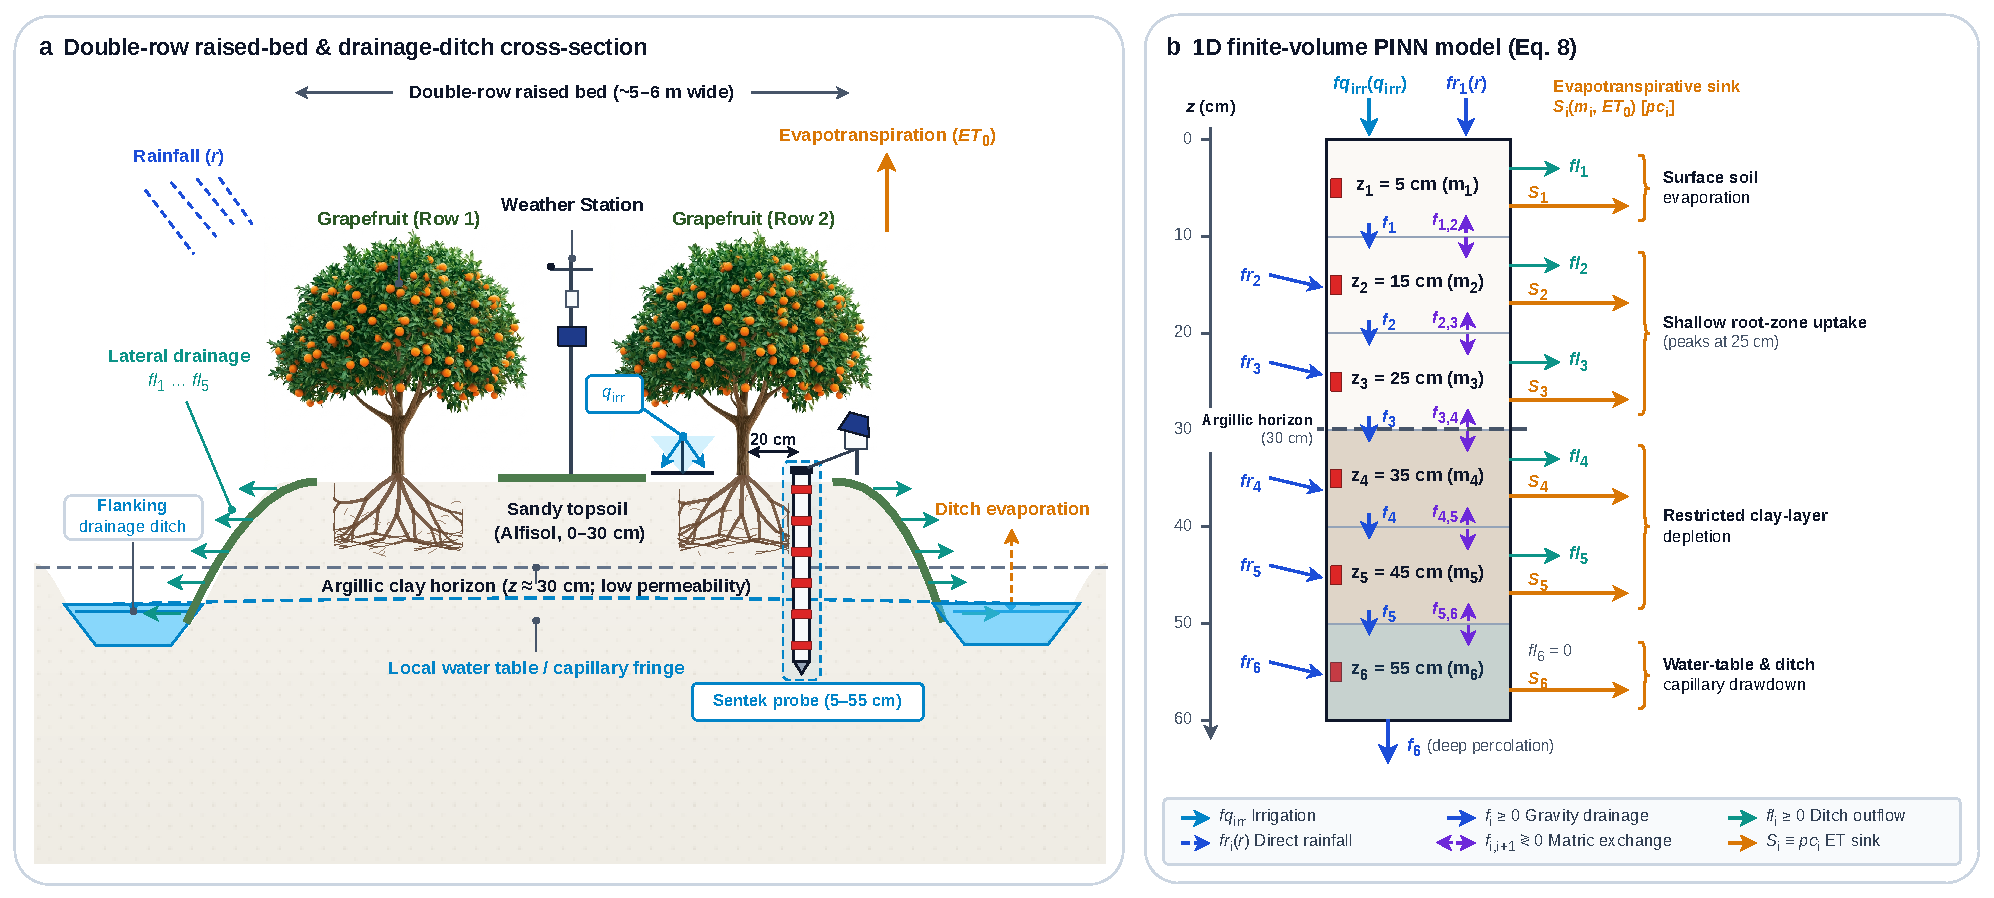
\includegraphics[width=0.92\linewidth]{bed_ditch_schematic.pdf}
\marginnote{R-1.4}\caption{\textcolor{blue}{Cross-sectional geometry (not to scale) of the IRREC Millennium Block experimental site (35-acre block; 20-acre active 5,500-tree citrus trial), showing a citrus tree planted on a raised sandy Alfisol bed flanked by drainage ditches above an argillic horizon at $\approx\SI{30}{cm}$ depth. A 6-depth Sentek Drill \& Drop capacitive probe (\SI{20}{cm} from the trunk) monitors 10-\si{cm} vertical compartments centered at 5, 15, 25, 35, 45, and 55~\si{cm}, alongside micro-sprinkler irrigation ($q_{\mathrm{irr}}$), rainfall ($r$), evapotranspiration ($ET_0$), vertical percolation ($f_i$), inter-layer exchange ($f_{i,i+1}$), and lateral ditch drainage ($fl_1\dots fl_5$).}}
\label{fig:bed_ditch}
\end{figure}

\begin{figure}[!htbp]
\centering
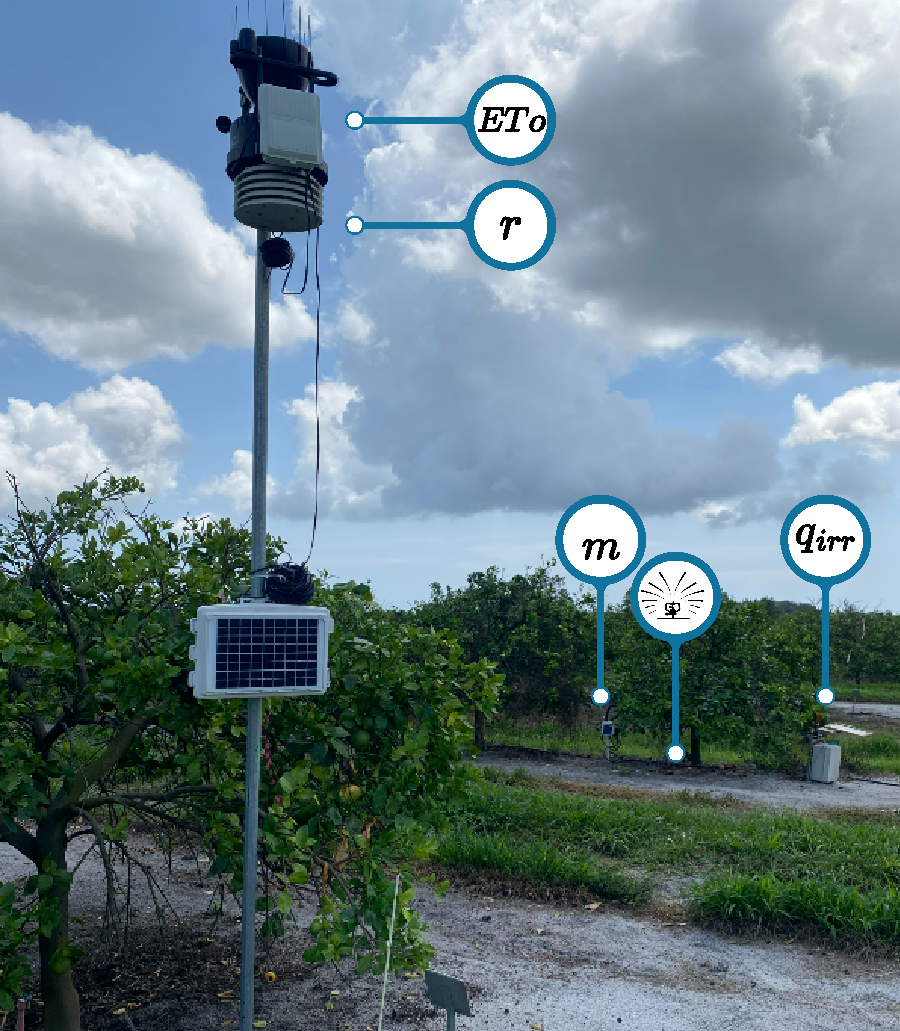
\includegraphics[width=0.5\linewidth]{sensorsmillenniumb.pdf}
\marginnote{R-1.10}\caption{Description of experimental setup, where a weather station, soil moisture probe, and irrigation sensor were deployed to collect soil moisture ($m$), rain ($r$), potential evapotranspiration ($ET_0$), and irrigation (\textcolor{blue}{$q_{\mathrm{irr}}$}) data.}
\label{sensorsmillennium}
\end{figure}

In a designated section of the Millennium Block, multiple sensors were installed (Fig. \ref{sensorsmillennium}), with data collected, processed, and stored using Irrigmonitor, a custom cloud-based application that facilitates real-time data integration for agricultural water management. The following instrumentation was deployed:
\begin{description}
\item[Weather Station:] A Davis Vantage Pro2 weather station\footnote{See \url{https://www.davisinstruments.com/pages/vantage-pro2} for more information on Davis weather stations.} providing rainfall \marginnote{R-1.2, R-1.10}\textcolor{blue}{(\si{mm/h})} and meteorological variables (temperature, humidity, wind speed, solar radiation, and barometric pressure). These data were employed to calculate $ET_0$ \textcolor{blue}{(\si{mm/h})} using the \textcolor{blue}{FAO-56} Penman--Monteith method \cite{allen1998crop}.
\item[Soil Moisture Probe:] SM measurements \textcolor{blue}{($m_1\dots m_6$ in \si{\%VWC})} were taken at 5\si{cm}, 15\si{cm}, 25\si{cm}, 35\si{cm}, 45\si{cm}, 55\si{cm} using a Sentek Drill \& Drop probe\footnote{Series II Sentek Drill \& Drop probe, capable of measuring SM, temperature, and salinity at 10\si{cm} intervals. See \url{https://sentektechnologies.com/download/sentek-drill-drop-probe-manual/} for details.}, located 20\si{cm} from the base of the tree.
\item[Irrigation Sensor:] Irrigation events were detected by installing two electrodes at the supply irrigation point, connected to a Campbell Scientific CR1000X datalogger, where changes in electrical conduction were used to identify irrigation events and their duration (\textcolor{blue}{$q_{\mathrm{irr}} \in [0,1]$\,}\si{h/h}).
\end{description}

We collected \marginnote{R-2.4}\textcolor{blue}{840 hourly records spanning 839 elapsed hours ($\approx 35$~days)} of data from March 28, 2025, \textcolor{blue}{21:00:00} to May 2, 2025, 20:00:00, for training. This period included approximately seven distinct rain events (Fig. \ref{Mainfig}). The duration of the training window was selected to ensure a sufficient number of rain events, which are scarce compared to other variables, such as reference evapotranspiration, which changes continuously, or irrigation events, which can be controlled to generate data. Further research on optimizing the estimation window duration and addressing scenarios with limited rainfall is planned, but is beyond the scope of this study.
Additionally, we \marginnote{R-2.3, R-2.4}\textcolor{blue}{extracted} 72 \textcolor{blue}{elapsed} hours (3 days\textcolor{blue}{, 73 hourly records}) of data from May 3, 2025, 21:00:00 to May 6, 2025, 21:00:00, for validation \textcolor{blue}{(leaving a 25-hour separation buffer before the May~3 21:00:00 initial state $m(0)$, with the full 792 unseen hours through June~5, 2025 evaluated in Section~\ref{sec:benchmarks}). Held-out evaluations use observed station rainfall ($r$), $ET_0$, and irrigation ($q_{\mathrm{irr}}$) to isolate intrinsic model dynamics, whereas operational deployment replaces station weather with forecast feeds~\cite{NWS2024}.} This 3-day validation window aligns with the typical 3-day prediction horizon of weather forecast data from sources such as the National Weather Service \cite{NWS2024}, which can be integrated into the algorithm for predictive irrigation management. This duration assesses the approach's effectiveness in leveraging short-term weather forecasts for irrigation scheduling.
All data were processed and standardized to a one-hour sampling interval to match the temporal resolution of weather forecast data \cite{NWS2024}. This sampling interval was chosen as a constraint because although sensors can collect data at smaller temporal scales, irrigation management strategies that integrate weather forecasts must rely on the temporal resolution of available forecast data.

\subsection{Computational Tools and Algorithm Setup}
The PINN was implemented using TensorFlow 2.10, with 64-bit floating-point precision (\texttt{float64}) to promote numerical stability and accuracy. TensorFlow’s automatic differentiation (synthetic differentiation) was employed to compute gradients and embed physical constraints directly into the training process.
The numerical integration of the PINN’s differential equations was performed using a custom RK4 solver \marginnote{R-2.9}\textcolor{blue}{(\(\Delta t = \SI{1}{h}\))} fully integrated into TensorFlow’s computational graph\textcolor{blue}{. Randomness across initialization and uniform collocation sampling (\(M = 1{,}000\) points per step) was controlled using fixed seed \texttt{42} across Python, NumPy, and TensorFlow. Both stages used AMSGrad-Adam optimization with gradient norm/value clipping at 0.5 and staircase exponential decay (factor 0.9 every 1,000 steps): Stage~1 ran for 3,000 epochs starting from \(\eta_1 = \num{7.97e-5}\), and Stage~2 refined parameters via RK4 trajectory tracking for 1,000 epochs starting from \(\eta_2 = \num{5.0e-6}\)}.

% Source code: FINAL_SUBMISSION/code/pinn_training.py (derived from Pinparameb.py)
% Figures: FINAL_SUBMISSION/code/paper_figures.ipynb
% Optuna: optuna_stage1b.py (Stage 1, 200 trials), PINN_optuna_stage2.py (Stage 2, 30 trials)
Hyperparameter optimization was performed using Optuna 3.5, a Bayesian optimization framework, across 200 trials for Stage 1, each evaluated for 150 epochs using the derivative loss ($j_1$), followed by 30 trials for Stage 2. Key hyperparameters obtained included:
\begin{itemize}
\item Initial learning rate for Stage 1 ($\eta_1$): \num{7.97e-5} \textcolor{blue}{(and Stage 2 $\eta_2 = \num{5.0e-6}$)}.
\item Number of neurons per layer ($H$): 56 \textcolor{blue}{(with $2H = 112$ on two-input sink branches $S_i$)}.
\item Loss weight multipliers: $\lambda_{c_1} = \num{113982766}$, $\lambda_{c_2} = \num{1773295}$, and $\lambda_{c_3} = \num{126704656}$.
\end{itemize}

\FloatBarrier

\section*{Funding}
This research was supported by the United States - Israel Binational Agricultural Research and Development Fund (Grant ID IS-5774-25) and the Florida Department of Agriculture and Consumer Services (Grant ID 33200).

{\color{blue}\section*{Code availability}\marginnote{E-1.2}
All custom Python/TensorFlow code developed for this study---including the two-stage PINN training pipeline, branched flux-network definitions, custom \texttt{float64} RK4 solver, inference scripts, trained model weights, statistical verification utilities, and the complete benchmark, ablation, and physical admissibility evaluation scripts---is openly deposited in Zenodo at \url{https://doi.org/10.5281/zenodo.19446129}.

\section*{Data availability}
The complete raw and hourly processed field sensor datasets (weather station, multi-depth soil moisture probe, and irrigation conductance telemetry) supporting all training, 3-day benchmark, and rolling unseen-window analyses are publicly deposited in Zenodo at \url{https://doi.org/10.5281/zenodo.19446129}.

\section*{Author contributions}
G.C. conceived the methodology, developed the PINN software and numerical verification experiments, analyzed the field data, and drafted the manuscript. S.M.G. supervised the research, acquired funding, designed the irrigation monitoring infrastructure, and contributed to manuscript revision. J.I.P. contributed to the control-theoretic, system-identification, and optimization formulation and manuscript review. F.T.Z. managed the Millennium Block citrus experimental site, provided agronomic interpretation, and reviewed the manuscript. All authors read and approved the final manuscript.

\section*{Competing interests}
The authors declare no competing interests.}

\bibliography{PINN}% common bib file


\end{document}